\documentclass[a4paper,11pt]{article}

\usepackage[utf8]{inputenc}
\usepackage[
    left=1.2cm,
    right=1.2cm,
    top=0cm,
    bottom=1.5cm,
    footskip=1.0cm
]{geometry}

\usepackage{helvet}
\renewcommand{\familydefault}{\sfdefault}
\usepackage[T1]{fontenc}
\usepackage{graphicx}
\usepackage{xcolor}
\usepackage{amsmath}
\usepackage{amssymb}
\usepackage{pifont}
\usepackage{anyfontsize}
\usepackage{tikz}
\usetikzlibrary{calc,positioning,shapes.geometric,shadows,arrows.meta}
\usepackage[most]{tcolorbox}
\usepackage{enumitem}
\usepackage{fancyhdr}
\usepackage{tabularx}
\usepackage{colortbl}
\usepackage{hyperref}
\usepackage{array}
\usepackage{fontawesome5}

% Compatibility fallbacks for FontAwesome5 icon macros across compiler distributions
\providecommand{\faShieldAlt}{\faShield*}
\providecommand{\faMapMarkerAlt}{\faMapMarker*}
\providecommand{\faPhoneAlt}{\faPhone*}
\providecommand{\faMapMarkedAlt}{\faMapMarked*}
\providecommand{\faWhatsapp}{\faPhone*}
\providecommand{\faHandsHelping}{\faHands*}
\providecommand{\faTruckMoving}{\faTruck*}
\providecommand{\faTruckLoading}{\faTruck*}
\providecommand{\faClinicMedical}{\faHospital*}
\providecommand{\faUsersCog}{\faUsers*}
\providecommand{\faUserTie}{\faUser*}
\providecommand{\faUserCheck}{\faUserCheck}
\providecommand{\faUserShield}{\faUserShield}
\providecommand{\faUserGraduate}{\faUserGraduate}
\providecommand{\faHandHoldingHeart}{\faHandHoldingHeart}

% =========================================================================
% GRAPHICS PATH CONFIGURATION (Overleaf / TexPage / Local Compilers)
% -------------------------------------------------------------------------
% When compiling online on Overleaf or TexPage (https://texpage.com/):
%   - Upload your images into the 'images/' directory in the online project.
% When compiling or editing locally:
%   - Images reside in 'company-profile-images/' and 'images/'.
% The \graphicspath below searches both directories seamlessly.
% All \includegraphics commands reference 'images/<filename>' or '<filename>'.
% =========================================================================
\graphicspath{{images/}{./images/}{../images/}{company-profile-images/}{../company-profile-images/}{./}{../}}


% =================================================
% MAKHASWA BRAND PALETTE
% =================================================
\definecolor{mhnavy}{HTML}{082D5A}        % Primary Brand Deep Navy
\definecolor{mhnavy2}{HTML}{0C3A6D}       % Mid Corporate Navy
\definecolor{mhnavy3}{HTML}{124884}       % Accent Navy
\definecolor{mhblue}{HTML}{1A56A0}        % Crisp Corporate Blue
\definecolor{mhbluebright}{HTML}{0066CC}  % Bright Blue Accent
\definecolor{mhbluelight}{HTML}{F0F4FA}   % Soft Light Blue Background
\definecolor{mhteal}{HTML}{008080}        % Est. Badge Teal
\definecolor{mhgold}{HTML}{C8A951}        % Subtle Gold Keyline
\definecolor{mhoffwhite}{HTML}{F8FAFC}    % Clean Slate Off-White
\definecolor{mhlightgray}{HTML}{E2E8F0}   % Clean Minimal Border
\definecolor{mhtext}{HTML}{1E293B}        % Charcoal Dark Body Text
\definecolor{mhtextmuted}{HTML}{64748B}   % Slate Gray Subtitle Text

\pagecolor{white}
\color{mhtext}

% Hyperlink configuration
\hypersetup{
    colorlinks=true,
    linkcolor=mhnavy,
    urlcolor=mhnavy,
    citecolor=mhblue
}

% Top Header Section Banner (Fixed Absolute Alignment)
\newcommand{\sectionbanner}[2]{%
    \begin{tikzpicture}[remember picture, overlay]
        % Navy Banner Bar across full top width (3.5cm height)
        \fill[mhnavy] (current page.north west) rectangle ([yshift=-3.5cm]current page.north east);
        \fill[mhgold] ([yshift=-3.5cm]current page.north west) rectangle ([yshift=-3.38cm]current page.north east);

        % Title & Subtitle (Centered vertically inside the 3.5cm banner)
        \node[anchor=west, inner sep=0pt, text width=0.62\paperwidth] at ([xshift=1.2cm, yshift=-1.75cm]current page.north west) {
            {\fontsize{21pt}{25pt}\selectfont\bfseries\color{white} #1}\\[0.22cm]
            {\footnotesize\bfseries\color{mhbluelight} \MakeUppercase{#2}}
        };

        % Logo Box (Centered vertically to match the title)
        \node[anchor=east, inner sep=0pt] at ([xshift=-1.2cm, yshift=-1.75cm]current page.north east) {
            \begin{tcolorbox}[
                enhanced,
                colback=white,
                colframe=mhlightgray,
                boxrule=0.8pt,
                arc=3pt,
                boxsep=2pt,
                left=4pt, right=4pt, top=3pt, bottom=3pt,
                width=3.2cm,
                halign=center
            ]
                
\includegraphics[height=1.0cm, keepaspectratio]{images/logo.jpeg}
            \end{tcolorbox}
        };
    \end{tikzpicture}%
    \vspace*{3.8cm}% Clears the 3.5cm banner cleanly before body content starts
    \noindent
}

% Reusable small stat / feature card
\newcommand{\statcard}[4][0pt]{%
    \begin{tcolorbox}[
        enhanced, colback=white, colframe=mhlightgray, boxrule=0.8pt, arc=4pt,
        left=2pt, right=2pt, top=7pt, bottom=7pt, halign=center,
        enlarge top by=#1,
        borderline north={2.2pt}{0pt}{#2}
    ]
        {\fontsize{17pt}{19pt}\selectfont\bfseries\color{#2} #3}\\[2pt]
        {\fontsize{7pt}{9pt}\selectfont\color{mhtextmuted}\MakeUppercase{#4}}
    \end{tcolorbox}%
}

% Reusable service/discipline card
\newcommand{\servicecard}[2]{%
    \begin{tcolorbox}[
        enhanced, colback=mhoffwhite, colframe=mhlightgray, boxrule=0.8pt, arc=4pt,
        left=8pt, right=8pt, top=7pt, bottom=7pt,
        borderline west={2.6pt}{0pt}{mhblue}
    ]
        {\fontsize{10pt}{12pt}\selectfont\bfseries\color{mhnavy} #1}\\[2.5pt]
        {\fontsize{8.2pt}{11pt}\selectfont\color{mhtext} #2}
    \end{tcolorbox}%
}

% =================================================
% FOOTER CONFIGURATION
% =================================================
\pagestyle{fancy}
\fancyhf{}
\renewcommand{\headrulewidth}{0pt}
\fancyfoot[L]{
    \fontsize{8pt}{10pt}\selectfont\color{mhtextmuted}
    \textbf{Makhaswa Holdings (Pty) Ltd} \ $\bullet$ \ CIDB Grade 8 CE PE / 8 ME PE \ $\bullet$ \ Reg: K2017/307900/07
}
\fancyfoot[R]{
    \fontsize{8pt}{10pt}\selectfont\color{mhnavy}
    \textbf{\thepage}
}

\begin{document}

% =========================================================================
% PAGE 1 --- LIGHT MINIMALIST COVER PAGE
% =========================================================================
\begin{titlepage}
\thispagestyle{empty}

\begin{tikzpicture}[remember picture, overlay]
    % Clean Pure White Canvas
    \fill[white] (current page.north west) rectangle (current page.south east);

    % Main Centered Brand Block
    \node[anchor=center] at ([yshift=2.5cm]current page.center) {
        \begin{minipage}{0.85\paperwidth}
            \centering
            % Mounted Brand Emblem / Logo
            \begin{tcolorbox}[
                enhanced,
                colback=white,
                colframe=white,
                boxrule=0pt,
                arc=0pt,
                left=0pt, right=0pt, top=0pt, bottom=0pt,
                width=5.5cm,
                halign=center
            ]
                
\includegraphics[width=5.0cm, keepaspectratio]{images/logo.jpeg}
            \end{tcolorbox}

            \vspace{0.8cm}

            % Company Name Block (Perfect Horizontal Centering)
            \begin{tikzpicture}
                % Primary Company Name
                \node[anchor=center] (name) at (0,0) {
                    {\fontsize{40pt}{44pt}\selectfont\bfseries\color{mhnavy}MAKHASWA}
                };
                
                % Subtitle HOLDINGS
                \node[anchor=north, yshift=-0.12cm] (sub) at (name.south) {
                    {\fontsize{19pt}{23pt}\selectfont\bfseries\color{mhblue}\makebox[\width][s]{HOLDINGS}}
                };

                % EST. 2017 Circular Seal (Overlayed on Right so it does not affect horizontal centering)
                \coordinate (estcenter) at ([xshift=1.25cm, yshift=0.06cm]name.east);
                \fill[mhteal, overlay] (estcenter) circle (0.84cm);
                \draw[white, line width=1.4pt, overlay] (estcenter) circle (0.74cm);
                \node[overlay, text=white, align=center, inner sep=0pt] at (estcenter) {
                    {\fontsize{8.5pt}{10pt}\selectfont\bfseries\color{white}EST.}\\[2.5pt]
                    {\fontsize{12pt}{13.5pt}\selectfont\bfseries\color{white}2017}
                };

                % Level 1 BBBEE Badge below Holdings
                \node[anchor=north, yshift=-0.28cm] (bbbee) at (sub.south) {
                    \begin{tcolorbox}[
                        enhanced,
                        colback=mhnavy,
                        colframe=mhnavy,
                        boxrule=0pt,
                        arc=3pt,
                        left=10pt, right=10pt, top=3.5pt, bottom=3.5pt,
                        width=3.8cm,
                        halign=center
                    ]
                        {\fontsize{8pt}{10pt}\selectfont\bfseries\color{white}\faAward\ \ LEVEL 1 BBBEE}
                    \end{tcolorbox}
                };
            \end{tikzpicture}

            \vspace{0.8cm}

            % Centered Thin Accent Rule
            \textcolor{mhnavy}{\rule{4.5cm}{1.2pt}}

            \vspace{0.6cm}

            % Document Category & Year
            {\fontsize{10.5pt}{13pt}\selectfont\bfseries\color{mhblue}\MakeUppercase{Company Profile}}\\[0.25cm]
            {\fontsize{20pt}{24pt}\selectfont\bfseries\color{mhblue}2026}
        \end{minipage}
    };

    % Subtle bottom CIDB footer notation
    \node[anchor=south] at ([yshift=1.2cm]current page.south) {
        {\fontsize{8pt}{10pt}\selectfont\color{mhtextmuted}
        \faHardHat\ CIDB Grade 8 CE PE / 8 ME PE \ $\bullet$ \ \faBuilding\ NHBRC Class 5 \ $\bullet$ \ Reg: K2017/307900/07}
    };
\end{tikzpicture}
\end{titlepage}
\clearpage

% =========================================================================
% PAGE 2 --- CONTENTS + SPLIT FULL-BLEED IMAGE
% =========================================================================
\thispagestyle{empty}

\begin{tikzpicture}[remember picture, overlay]
    % ----------------------------------------------------
    % LEFT HALF: CONTENTS LISTING (50% Canvas)
    % ----------------------------------------------------
    \fill[white] (current page.north west) rectangle ([xshift=0.50\paperwidth]current page.south west);

    \node[anchor=north west, inner sep=0pt] at ([xshift=1.2cm, yshift=-1.5cm]current page.north west) {
        \begin{minipage}{0.42\paperwidth}
            {\fontsize{24pt}{28pt}\selectfont\bfseries\color{mhblue}Contents}
            \vspace{0.5cm}

            \fontsize{8.2pt}{13.8pt}\selectfont

            \noindent
            {\bfseries\color{mhblue}01\ \ Executive Summary \& National Footprint} \dotfill {\bfseries\color{mhnavy}1}\\[2pt]
            {\bfseries\color{mhblue}02\ \ Governance, Leadership \& CR Appointments} \dotfill {\bfseries\color{mhnavy}2}\\[2pt]
            {\bfseries\color{mhblue}03\ \ Statutory Registrations \& CIDB Matrix} \dotfill {\bfseries\color{mhnavy}3}\\[2pt]
            {\bfseries\color{mhblue}04\ \ Our Journey \& Strategic Milestones} \dotfill {\bfseries\color{mhnavy}4}\\[2pt]
            {\bfseries\color{mhblue}05\ \ Core Engineering Disciplines \& Capabilities} \dotfill {\bfseries\color{mhnavy}5}\\[2pt]
            {\bfseries\color{mhblue}06\ \ Plant, Fleet \& Technical Software Capacity} \dotfill {\bfseries\color{mhnavy}6}\\[2pt]
            {\bfseries\color{mhblue}07\ \ SHEQ Policy, ISO Alignment \& Lab Testing} \dotfill {\bfseries\color{mhnavy}7}\\[2pt]
            {\bfseries\color{mhblue}08\ \ Project Portfolio: Civil Infrastructure \& Roads} \dotfill {\bfseries\color{mhnavy}8}\\[2pt]
            {\bfseries\color{mhblue}09\ \ Project Portfolio: Buildings, Water \& Reticulation} \dotfill {\bfseries\color{mhnavy}9}\\[2pt]
            {\bfseries\color{mhblue}10\ \ CSI \& Socio-Economic Transformation} \dotfill {\bfseries\color{mhnavy}10}\\[2pt]
            {\bfseries\color{mhblue}11\ \ Contactable References Directory} \dotfill {\bfseries\color{mhnavy}11}\\[2pt]
            {\bfseries\color{mhblue}12\ \ Tender Due Diligence, Warranties \& Contacts} \dotfill {\bfseries\color{mhnavy}12}

            \vspace{0.4cm}
            \textcolor{mhlightgray}{\rule{\linewidth}{0.8pt}}
            \vspace{0.25cm}

            {\fontsize{7.5pt}{10.5pt}\selectfont\color{mhtextmuted}
            \textbf{Makhaswa Holdings (Pty) Ltd} $\bullet$ Reg: 2017/307900/07\\
            CIDB Grade 8 CE PE / 8 ME PE $\bullet$ Level 1 B-BBEE
            }
        \end{minipage}
    };

    % ----------------------------------------------------
    % RIGHT HALF: FULL-BLEED ARCHITECTURAL PHOTO
    % ----------------------------------------------------
    \node[anchor=north east, inner sep=0pt] at (current page.north east) {
        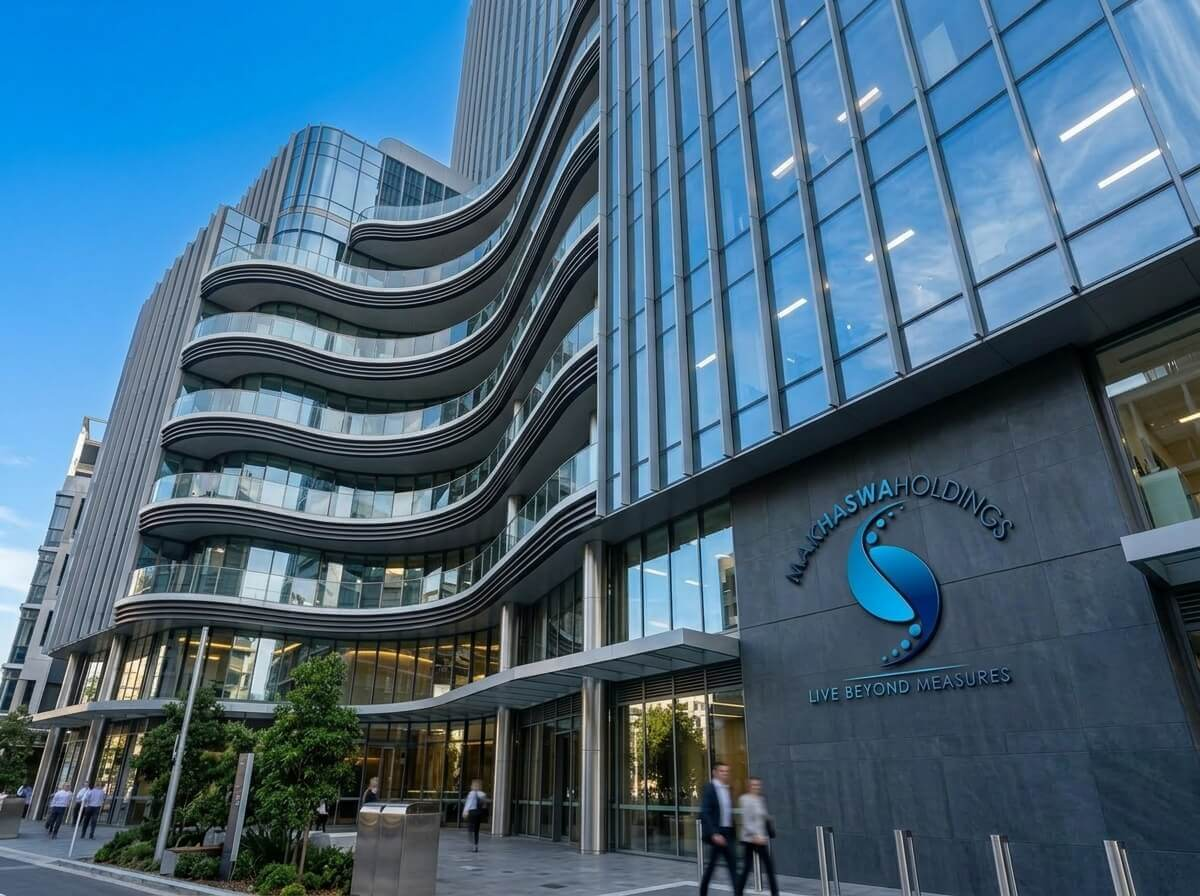
\includegraphics[width=0.50\paperwidth, height=\paperheight, keepaspectratio=false]{images/makhaswa-building-hero.jpeg}
    };

    % Small Right Page Number
    \node[anchor=south east, inner sep=0pt] at ([xshift=-0.8cm, yshift=0.8cm]current page.south east) {
        {\fontsize{9pt}{10pt}\selectfont\bfseries\color{white}2}
    };
\end{tikzpicture}
\clearpage

% Reset page numbering so the footer counter matches the Overview TOC (content = page 1)
\setcounter{page}{1}

% =================================================
% PAGE 4 (CONTENT p.1) --- EXECUTIVE SUMMARY & NATIONAL FOOTPRINT
% =================================================

\sectionbanner{EXECUTIVE OVERVIEW}{Corporate Identity, Strategic Vision \& National Footprint}

\noindent
\begin{minipage}[t]{0.62\textwidth}
    {\large\bfseries\color{mhnavy} Who We Are}
    \vspace{0.15cm}

    {\fontsize{9pt}{12.8pt}\selectfont\color{mhtext}
    \textbf{Makhaswa Holdings (Pty) Ltd} is a premier, 100\% Black-Owned, Level 1 B-BBEE multi-disciplinary civil engineering, infrastructure development, mechanical, and general building construction enterprise headquartered in Pretoria, Gauteng. The company was officially incorporated with the Companies and Intellectual Property Commission (CIPC) on \textbf{17 July 2017} (Registration: \textbf{2017/307900/07}).
    }

    \vspace{0.25cm}

    {\fontsize{9pt}{12.8pt}\selectfont\color{mhtext}
    Through continuous capital investment and flawless project execution, Makhaswa Holdings has scaled into an elite contractor holding top-tier \textbf{CIDB Grade 8 CE PE} (Civil Engineering) and \textbf{8 ME PE} (Mechanical Engineering) ratings, alongside active accreditations in Specialist Building (7SB PE), Electrical Infrastructure (7EB PE), and General Building (6GB PE).
    }

    \vspace{0.25cm}

    {\fontsize{9pt}{12.8pt}\selectfont\color{mhtext}
    We execute public infrastructure tenders, municipal framework contracts, commercial facilities, and bulk reticulation schemes across Gauteng, Limpopo, KwaZulu-Natal, and North West.
    }
\end{minipage}
\hfill
\begin{minipage}[t]{0.34\textwidth}
    % Credentials Stat Container
    \begin{tcolorbox}[
        enhanced,
        colback=mhoffwhite,
        colframe=mhnavy,
        boxrule=1pt,
        arc=4pt,
        title={\bfseries\color{white} Key Accreditations},
        colbacktitle=mhnavy,
        left=7pt, right=7pt, top=6pt, bottom=6pt
    ]
        \fontsize{8pt}{11pt}\selectfont
        \textcolor{mhnavy}{\rule{4pt}{4pt}}\hspace{4pt}\textbf{CIDB Grade 8 CE PE / 8 ME PE}\\
        \textcolor{mhnavy}{\rule{4pt}{4pt}}\hspace{4pt}\textbf{CIDB 7SB PE / 7EB PE / 6GB PE}\\
        \textcolor{mhnavy}{\rule{4pt}{4pt}}\hspace{4pt}\textbf{Level 1 B-BBEE (135\% Recognition)}\\
        \textcolor{mhnavy}{\rule{4pt}{4pt}}\hspace{4pt}\textbf{NHBRC Registered (Class 5 Builder)}\\
        \textcolor{mhnavy}{\rule{4pt}{4pt}}\hspace{4pt}\textbf{ISO 9001 $\bullet$ 14001 $\bullet$ 45001}
    \end{tcolorbox}

    \vspace{0.25cm}

    \begin{tcolorbox}[
        enhanced, colback=white, colframe=mhlightgray, boxrule=0.8pt, arc=4pt,
        left=6pt, right=6pt, top=6pt, bottom=6pt, halign=center
    ]
        {\fontsize{18pt}{20pt}\selectfont\bfseries\color{mhblue} 2017}\\[1pt]
        {\fontsize{7.5pt}{9pt}\selectfont\color{mhtextmuted}\MakeUppercase{Incorporated July 2017}}\\[4pt]
        \textcolor{mhlightgray}{\rule{3.2cm}{0.6pt}}\\[4pt]
        {\fontsize{18pt}{20pt}\selectfont\bfseries\color{mhblue} 100\%}\\[1pt]
        {\fontsize{7.5pt}{9pt}\selectfont\color{mhtextmuted}\MakeUppercase{Black Owned / 50\% Female}}
    \end{tcolorbox}
\end{minipage}

\vspace{0.3cm}

% Vision & Mission Split Cards
\noindent
\begin{minipage}[t]{0.485\textwidth}
    \begin{tcolorbox}[
        enhanced, colback=white, colframe=mhlightgray, boxrule=0.8pt, arc=4pt,
        title={\bfseries\color{mhnavy} Our Vision},
        colbacktitle=mhoffwhite, coltitle=mhnavy, fonttitle=\bfseries\small,
        left=8pt, right=8pt, top=7pt, bottom=7pt,
        borderline west={3pt}{0pt}{mhnavy}
    ]
        {\fontsize{8.5pt}{11.5pt}\selectfont\color{mhtext}
        To be a leading African infrastructure and engineering contractor recognized for execution excellence, innovative engineering solutions, uncompromised safety standards, and sustainable socio-economic development.
        }
    \end{tcolorbox}
\end{minipage}
\hfill
\begin{minipage}[t]{0.485\textwidth}
    \begin{tcolorbox}[
        enhanced, colback=white, colframe=mhlightgray, boxrule=0.8pt, arc=4pt,
        title={\bfseries\color{mhnavy} Our Mission},
        colbacktitle=mhoffwhite, coltitle=mhnavy, fonttitle=\bfseries\small,
        left=8pt, right=8pt, top=7pt, bottom=7pt,
        borderline west={3pt}{0pt}{mhblue}
    ]
        {\fontsize{8.5pt}{11.5pt}\selectfont\color{mhtext}
        To procure and execute construction projects at competitive pricing, provide safe working environments, deliver quality infrastructure on time and within budget, and empower local communities through skills transfer.
        }
    \end{tcolorbox}
\end{minipage}

\vspace{0.25cm}

% Core Values Strip
\noindent
{\large\bfseries\color{mhnavy} Core Corporate Values}
\vspace{0.15cm}

\noindent
\begin{minipage}[t]{0.155\textwidth}\statcard{mhnavy}{01}{Integrity}\end{minipage}\hfill
\begin{minipage}[t]{0.155\textwidth}\statcard[10pt]{mhblue}{02}{Excellence}\end{minipage}\hfill
\begin{minipage}[t]{0.155\textwidth}\statcard{mhbluebright}{03}{Safety 1st}\end{minipage}\hfill
\begin{minipage}[t]{0.155\textwidth}\statcard[10pt]{mhnavy3}{04}{Empowerment}\end{minipage}\hfill
\begin{minipage}[t]{0.155\textwidth}\statcard{mhblue}{05}{Sustainability}\end{minipage}\hfill
\begin{minipage}[t]{0.155\textwidth}\statcard[10pt]{mhnavy}{06}{Governance}\end{minipage}

\vspace{0.25cm}

% National Regional Footprint Mini Strip
\noindent
\begin{tcolorbox}[
    enhanced, colback=mhoffwhite, colframe=mhlightgray, boxrule=0.7pt, arc=4pt,
    left=8pt, right=8pt, top=6pt, bottom=6pt
]
    \fontsize{8pt}{10.5pt}\selectfont
    \textbf{\color{mhnavy}Regional Operational Footprint:} \
    \textbf{Pretoria HQ:} 869 Patryshond St, Garsfontein \ $\bullet$ \
    \textbf{Midrand Logistics:} Riversands Incubation Hub \ $\bullet$ \
    \textbf{Limpopo Hub:} 197 Dudu Madisha Dr, Mokopane \ $\bullet$ \
    \textbf{KZN Hub:} 71 Bertha Mkhize St, Durban Central
\end{tcolorbox}

\clearpage

% =================================================
% PAGE 5 (CONTENT p.2) --- GOVERNANCE, LEADERSHIP & STATUTORY APPOINTMENTS
% =================================================

\sectionbanner{GOVERNANCE \& LEADERSHIP}{Executive Management \& Statutory CR Appointments}

\noindent
\begin{minipage}[t]{0.485\textwidth}
    \begin{tcolorbox}[
        enhanced, colback=white, colframe=mhlightgray, boxrule=0.8pt, arc=4pt,
        left=8pt, right=8pt, top=8pt, bottom=8pt,
        borderline west={3.5pt}{0pt}{mhnavy}
    ]
        {\fontsize{10pt}{12pt}\selectfont\bfseries\color{mhnavy}Lucas Dinga} \ \ {\fontsize{8pt}{10pt}\selectfont\color{mhtextmuted}(CEO / Authorized Signatory)}\\[2pt]
        {\fontsize{7.8pt}{9.5pt}\selectfont\bfseries\color{mhblue}Statutory CR 7(19c) Appointee}\\[4pt]
        {\fontsize{8.2pt}{11pt}\selectfont\color{mhtext}
        Oversees corporate strategy, commercial expansion, tender procurement, joint ventures, and client relations. Brings over 10 years of specialised experience in civil engineering, road works, and major building contracts. Sole designated signatory for legal contracts and financial operations.
        }
    \end{tcolorbox}
\end{minipage}
\hfill
\begin{minipage}[t]{0.485\textwidth}
    \begin{tcolorbox}[
        enhanced, colback=white, colframe=mhlightgray, boxrule=0.8pt, arc=4pt,
        left=8pt, right=8pt, top=8pt, bottom=8pt,
        borderline west={3.5pt}{0pt}{mhblue}
    ]
        {\fontsize{10pt}{12pt}\selectfont\bfseries\color{mhnavy}Nelly Motswapong (Ms. Nelly)} \ \ {\fontsize{8pt}{10pt}\selectfont\color{mhtextmuted}(Director / Co-Owner)}\\[2pt]
        {\fontsize{7.8pt}{9.5pt}\selectfont\bfseries\color{mhblue}50\% Black Female Ownership Equity}\\[4pt]
        {\fontsize{8.2pt}{11pt}\selectfont\color{mhtext}
        Directs corporate governance, human capital development, broad-based enterprise transformation, CSI initiatives, and operational administration. Ensures that all site operations adhere strictly to employment equity and community upliftment mandates.
        }
    \end{tcolorbox}
\end{minipage}

\vspace{0.25cm}

{\large\bfseries\color{mhnavy} Statutory Appointments (OHS Act 85 of 1993 \& Construction Regulations 2014)}
\vspace{0.15cm}

\noindent
{\fontsize{8.2pt}{10.8pt}\selectfont\color{mhtext}
All site and executive operations are strictly structured in full compliance with the Occupational Health and Safety Act and the Construction Regulations 2014, backed by certified professional personnel:
}

\vspace{0.2cm}

\renewcommand{\arraystretch}{1.3}
\begin{tabularx}{\textwidth}{@{}p{3.8cm} p{3.4cm} p{2.2cm} X@{}}
\rowcolor{mhnavy}
{\color{white}\bfseries\fontsize{8pt}{10pt}\selectfont Key Personnel} &
{\color{white}\bfseries\fontsize{8pt}{10pt}\selectfont Designation} &
{\color{white}\bfseries\fontsize{8pt}{10pt}\selectfont Statutory Ref} &
{\color{white}\bfseries\fontsize{8pt}{10pt}\selectfont Primary Operational Responsibility} \\
\rowcolor{mhbluelight}
\fontsize{7.8pt}{9.5pt}\selectfont\bfseries Lucas Dinga & \fontsize{7.8pt}{9.5pt}\selectfont Chief Executive Officer & \fontsize{7.8pt}{9.5pt}\selectfont CR 7(19c) & \fontsize{7.8pt}{9.5pt}\selectfont Corporate leadership, commercial sign-off, tender bids \\
\fontsize{7.8pt}{9.5pt}\selectfont\bfseries Elphas Goodman Mdaka & \fontsize{7.8pt}{9.5pt}\selectfont Project \& Contracts Manager & \fontsize{7.8pt}{9.5pt}\selectfont CR 16.2 \& 8.1 & \fontsize{7.8pt}{9.5pt}\selectfont Contractual administration, client liaison (074 481 0520) \\
\rowcolor{mhbluelight}
\fontsize{7.8pt}{9.5pt}\selectfont\bfseries Peter Makwela & \fontsize{7.8pt}{9.5pt}\selectfont Construction Manager & \fontsize{7.8pt}{9.5pt}\selectfont CR 16.2 \& 8.1 & \fontsize{7.8pt}{9.5pt}\selectfont Multi-site programming, fleet dispatch \& logistics \\
\fontsize{7.8pt}{9.5pt}\selectfont\bfseries Sfiso Knowledge Nkabinde & \fontsize{7.8pt}{9.5pt}\selectfont Construction Manager / Site Agent & \fontsize{7.8pt}{9.5pt}\selectfont CR 8.1 & \fontsize{7.8pt}{9.5pt}\selectfont Day-to-day site management, resource execution \\
\rowcolor{mhbluelight}
\fontsize{7.8pt}{9.5pt}\selectfont\bfseries Lindelani Shangase & \fontsize{7.8pt}{9.5pt}\selectfont SHEQ Officer & \fontsize{7.8pt}{9.5pt}\selectfont CR 8.5 (Pr.OHS) & \fontsize{7.8pt}{9.5pt}\selectfont Health \& Safety audits, environmental compliance \\
\fontsize{7.8pt}{9.5pt}\selectfont\bfseries Hendrick Chauke & \fontsize{7.8pt}{9.5pt}\selectfont Quality Controller (QC) & \fontsize{7.8pt}{9.5pt}\selectfont CR 8.38 & \fontsize{7.8pt}{9.5pt}\selectfont ITPs, slump tests, concrete 28-day cube crushing \\
\rowcolor{mhbluelight}
\fontsize{7.8pt}{9.5pt}\selectfont\bfseries Henry Chauke & \fontsize{7.8pt}{9.5pt}\selectfont Section Supervisor & \fontsize{7.8pt}{9.5pt}\selectfont CR 8.8 & \fontsize{7.8pt}{9.5pt}\selectfont Section layerworks, pipelaying, structural builds \\
\fontsize{7.8pt}{9.5pt}\selectfont\bfseries Fulufhelo Shidade & \fontsize{7.8pt}{9.5pt}\selectfont Assistant Supervisor / Foreman & \fontsize{7.8pt}{9.5pt}\selectfont CR 8.7 & \fontsize{7.8pt}{9.5pt}\selectfont Front-line task supervision, artisan gang coordination \\
\rowcolor{mhbluelight}
\fontsize{7.8pt}{9.5pt}\selectfont\bfseries Thabiso Paul Mabetoa & \fontsize{7.8pt}{9.5pt}\selectfont Safety Representative & \fontsize{7.8pt}{9.5pt}\selectfont CR 17.1 & \fontsize{7.8pt}{9.5pt}\selectfont Daily toolbox talks, PPE enforcement, hazard logs \\
\fontsize{7.8pt}{9.5pt}\selectfont\bfseries C. Mazarura & \fontsize{7.8pt}{9.5pt}\selectfont Professional Land Surveyor & \fontsize{7.8pt}{9.5pt}\selectfont Pr.L.S. & \fontsize{7.8pt}{9.5pt}\selectfont Setting out, GPS road profiling, as-built coordinates \\
\end{tabularx}
\renewcommand{\arraystretch}{1}

\vspace{0.25cm}

% Workforce Capacity Card
\noindent
\begin{tcolorbox}[
    enhanced, colback=mhoffwhite, colframe=mhnavy, boxrule=0.9pt, arc=4pt,
    left=9pt, right=9pt, top=6pt, bottom=6pt
]
    \fontsize{8pt}{11pt}\selectfont\color{mhtext}
    \textbf{\color{mhnavy}Workforce Capacity \& Scalability:} Makhaswa Holdings maintains a core permanent workforce of civil engineers, project managers, survey technicians, certified machine operators, and skilled artisans, scaling to \textbf{100 -- 200 personnel} across active project teams with structured local community labour recruitment.
\end{tcolorbox}

\clearpage

% =================================================
% PAGE 6 (CONTENT p.3) --- STATUTORY REGISTRATIONS, ACCREDITATIONS & CIDB MATRIX
% =================================================

\sectionbanner{ACCREDITATIONS}{CIDB Grading Matrix, Statutory Registrations \& Banking}

\noindent
{\fontsize{9pt}{12.5pt}\selectfont\color{mhtext}
Makhaswa Holdings maintains full statutory and professional compliance across every regulatory authority governing South African construction. All registrations are active and verifiable for tender due diligence:
}

\vspace{0.25cm}

% Accreditation Badges Grid (5 Official Badges)
\noindent
\begin{minipage}[t]{0.185\textwidth}
    \begin{tcolorbox}[
        enhanced, colback=white, colframe=mhlightgray, boxrule=0.8pt, arc=4pt,
        halign=center, valign=center, left=2pt, right=2pt, top=3pt, bottom=3pt, height=2.2cm
    ]
        
\includegraphics[width=\linewidth, height=1.15cm, keepaspectratio]{images/cidb-logo.png}\\[1pt]
        {\fontsize{7pt}{8pt}\selectfont\bfseries\color{mhnavy}CIDB Grade 8}
    \end{tcolorbox}
\end{minipage}\hfill
\begin{minipage}[t]{0.185\textwidth}
    \begin{tcolorbox}[
        enhanced, colback=white, colframe=mhlightgray, boxrule=0.8pt, arc=4pt,
        halign=center, valign=center, left=2pt, right=2pt, top=3pt, bottom=3pt, height=2.2cm
    ]
        
\includegraphics[width=\linewidth, height=1.15cm, keepaspectratio]{images/bbbee-logo.png}\\[1pt]
        {\fontsize{7pt}{8pt}\selectfont\bfseries\color{mhnavy}Level 1 B-BBEE}
    \end{tcolorbox}
\end{minipage}\hfill
\begin{minipage}[t]{0.185\textwidth}
    \begin{tcolorbox}[
        enhanced, colback=white, colframe=mhlightgray, boxrule=0.8pt, arc=4pt,
        halign=center, valign=center, left=2pt, right=2pt, top=3pt, bottom=3pt, height=2.2cm
    ]
        
\includegraphics[width=\linewidth, height=1.15cm, keepaspectratio]{images/iso-logo.png}\\[1pt]
        {\fontsize{7pt}{8pt}\selectfont\bfseries\color{mhnavy}ISO 9001/14001/45001}
    \end{tcolorbox}
\end{minipage}\hfill
\begin{minipage}[t]{0.185\textwidth}
    \begin{tcolorbox}[
        enhanced, colback=white, colframe=mhlightgray, boxrule=0.8pt, arc=4pt,
        halign=center, valign=center, left=2pt, right=2pt, top=3pt, bottom=3pt, height=2.2cm
    ]
        
\includegraphics[width=\linewidth, height=1.15cm, keepaspectratio]{images/nhbrc-logo.png}\\[1pt]
        {\fontsize{7pt}{8pt}\selectfont\bfseries\color{mhnavy}NHBRC Class 5}
    \end{tcolorbox}
\end{minipage}\hfill
\begin{minipage}[t]{0.185\textwidth}
    \begin{tcolorbox}[
        enhanced, colback=white, colframe=mhlightgray, boxrule=0.8pt, arc=4pt,
        halign=center, valign=center, left=2pt, right=2pt, top=3pt, bottom=3pt, height=2.2cm
    ]
        
\includegraphics[width=\linewidth, height=1.15cm, keepaspectratio]{images/sheq-logo.png}\\[1pt]
        {\fontsize{7pt}{8pt}\selectfont\bfseries\color{mhnavy}SHEQ Framework}
    \end{tcolorbox}
\end{minipage}

\vspace{0.25cm}

% CIDB Grading Matrix Table
{\large\bfseries\color{mhnavy} CIDB Multi-Disciplinary Grading Matrix (CRS No: 10153817)}
\vspace{0.15cm}

\renewcommand{\arraystretch}{1.25}
\begin{tabularx}{\textwidth}{@{}p{2.5cm} p{7.0cm} X@{}}
\rowcolor{mhnavy}
{\color{white}\bfseries\fontsize{8pt}{10pt}\selectfont CIDB Grade} &
{\color{white}\bfseries\fontsize{8pt}{10pt}\selectfont Engineering Class / Discipline} &
{\color{white}\bfseries\fontsize{8pt}{10pt}\selectfont Tender Value Capability} \\
\rowcolor{mhbluelight}
\fontsize{8pt}{10pt}\selectfont\bfseries 8 CE PE & \fontsize{8pt}{10pt}\selectfont Civil Engineering Works (Potentially Emerging) & \fontsize{8pt}{10pt}\selectfont\bfseries Up to R200 Million \\
\fontsize{8pt}{10pt}\selectfont\bfseries 8 ME PE & \fontsize{8pt}{10pt}\selectfont Mechanical Engineering Infrastructure & \fontsize{8pt}{10pt}\selectfont\bfseries Up to R200 Million \\
\rowcolor{mhbluelight}
\fontsize{8pt}{10pt}\selectfont\bfseries 7 SB PE & \fontsize{8pt}{10pt}\selectfont Specialist Building Works & \fontsize{8pt}{10pt}\selectfont\bfseries Up to R60 Million \\
\fontsize{8pt}{10pt}\selectfont\bfseries 7 EB PE & \fontsize{8pt}{10pt}\selectfont Electrical Engineering Works (Building) & \fontsize{8pt}{10pt}\selectfont\bfseries Up to R60 Million \\
\rowcolor{mhbluelight}
\fontsize{8pt}{10pt}\selectfont\bfseries 6 GB PE & \fontsize{8pt}{10pt}\selectfont General Building Works & \fontsize{8pt}{10pt}\selectfont\bfseries Up to R30 Million \\
\end{tabularx}
\renewcommand{\arraystretch}{1}

\vspace{0.25cm}

% Full Statutory Registrations Table
{\large\bfseries\color{mhnavy} Statutory Compliance \& Vendor Registrations}
\vspace{0.15cm}

\renewcommand{\arraystretch}{1.2}
\begin{tabularx}{\textwidth}{@{}p{4.8cm} X@{}}
\rowcolor{mhnavy}
{\color{white}\bfseries\fontsize{8pt}{10pt}\selectfont Compliance Parameter} & {\color{white}\bfseries\fontsize{8pt}{10pt}\selectfont Official Corporate Record} \\
\rowcolor{mhbluelight}
\fontsize{7.8pt}{9.5pt}\selectfont\bfseries CIPC Registration Number & \fontsize{7.8pt}{9.5pt}\selectfont 2017/307900/07 (Incorporated 17 July 2017) \\
\fontsize{7.8pt}{9.5pt}\selectfont\bfseries B-BBEE Contributor Status & \fontsize{7.8pt}{9.5pt}\selectfont Level 1 Contributor (135\% Procurement Recognition $\bullet$ 100\% Black Owned) \\
\rowcolor{mhbluelight}
\fontsize{7.8pt}{9.5pt}\selectfont\bfseries National Treasury CSD Supplier No. & \fontsize{7.8pt}{9.5pt}\selectfont MAAA0584716 (Master Supplier Database Verified) \\
\fontsize{7.8pt}{9.5pt}\selectfont\bfseries NHBRC Home Builder Number & \fontsize{7.8pt}{9.5pt}\selectfont 4000006217 (Provisional Class 5 Registered Home Builder) \\
\rowcolor{mhbluelight}
\fontsize{7.8pt}{9.5pt}\selectfont\bfseries SARS Tax Numbers & \fontsize{7.8pt}{9.5pt}\selectfont Income Tax: 9670117176 \ $\bullet$ \ VAT Registration: 4840286027 \\
\fontsize{7.8pt}{9.5pt}\selectfont\bfseries COIDA \& UIF Numbers & \fontsize{7.8pt}{9.5pt}\selectfont COIDA: 990001157115 (Letter of Good Standing) \ $\bullet$ \ UIF: 2577464/8 \\
\rowcolor{mhbluelight}
\fontsize{7.8pt}{9.5pt}\selectfont\bfseries Municipal Vendor Numbers & \fontsize{7.8pt}{9.5pt}\selectfont City of Johannesburg (CoJ): 125166 \ $\bullet$ \ Gauteng Province (GPG): 11000148444 \\
\fontsize{7.8pt}{9.5pt}\selectfont\bfseries Verified Corporate Banking & \fontsize{7.8pt}{9.5pt}\selectfont First National Bank (FNB) | Cheque Acc: 62763534445 | Branch: 251445 \\
\end{tabularx}
\renewcommand{\arraystretch}{1}

\vspace{0.25cm}

\noindent
\begin{minipage}[t]{0.235\textwidth}\statcard{mhnavy}{L1}{B-BBEE Level}\end{minipage}\hfill
\begin{minipage}[t]{0.235\textwidth}\statcard{mhblue}{8 CE/ME}{CIDB Grade}\end{minipage}\hfill
\begin{minipage}[t]{0.235\textwidth}\statcard{mhbluebright}{100\%}{Black-Owned}\end{minipage}\hfill
\begin{minipage}[t]{0.235\textwidth}\statcard{mhnavy3}{3x}{ISO Standards}\end{minipage}

\clearpage

% =================================================
% PAGE 7 (CONTENT p.4) --- OUR JOURNEY (KEY MILESTONES & STRATEGIC TRAJECTORY)
% =================================================

\sectionbanner{OUR JOURNEY}{Strategic Growth, Key Milestones \& Track Record}

\noindent
{\fontsize{9.2pt}{13pt}\selectfont\color{mhtext}
\textbf{Established in 2017}, Makhaswa Holdings (Pty) Ltd has charted an exponential growth trajectory from early civils in Gauteng to a nationally active, Tier-1 contractor executing mega-infrastructure across four provinces:
}

\vspace{0.25cm}

% =========================================================
% ALTERNATING LEFT-RIGHT TIMELINE ROADMAP
% =========================================================
\begin{center}
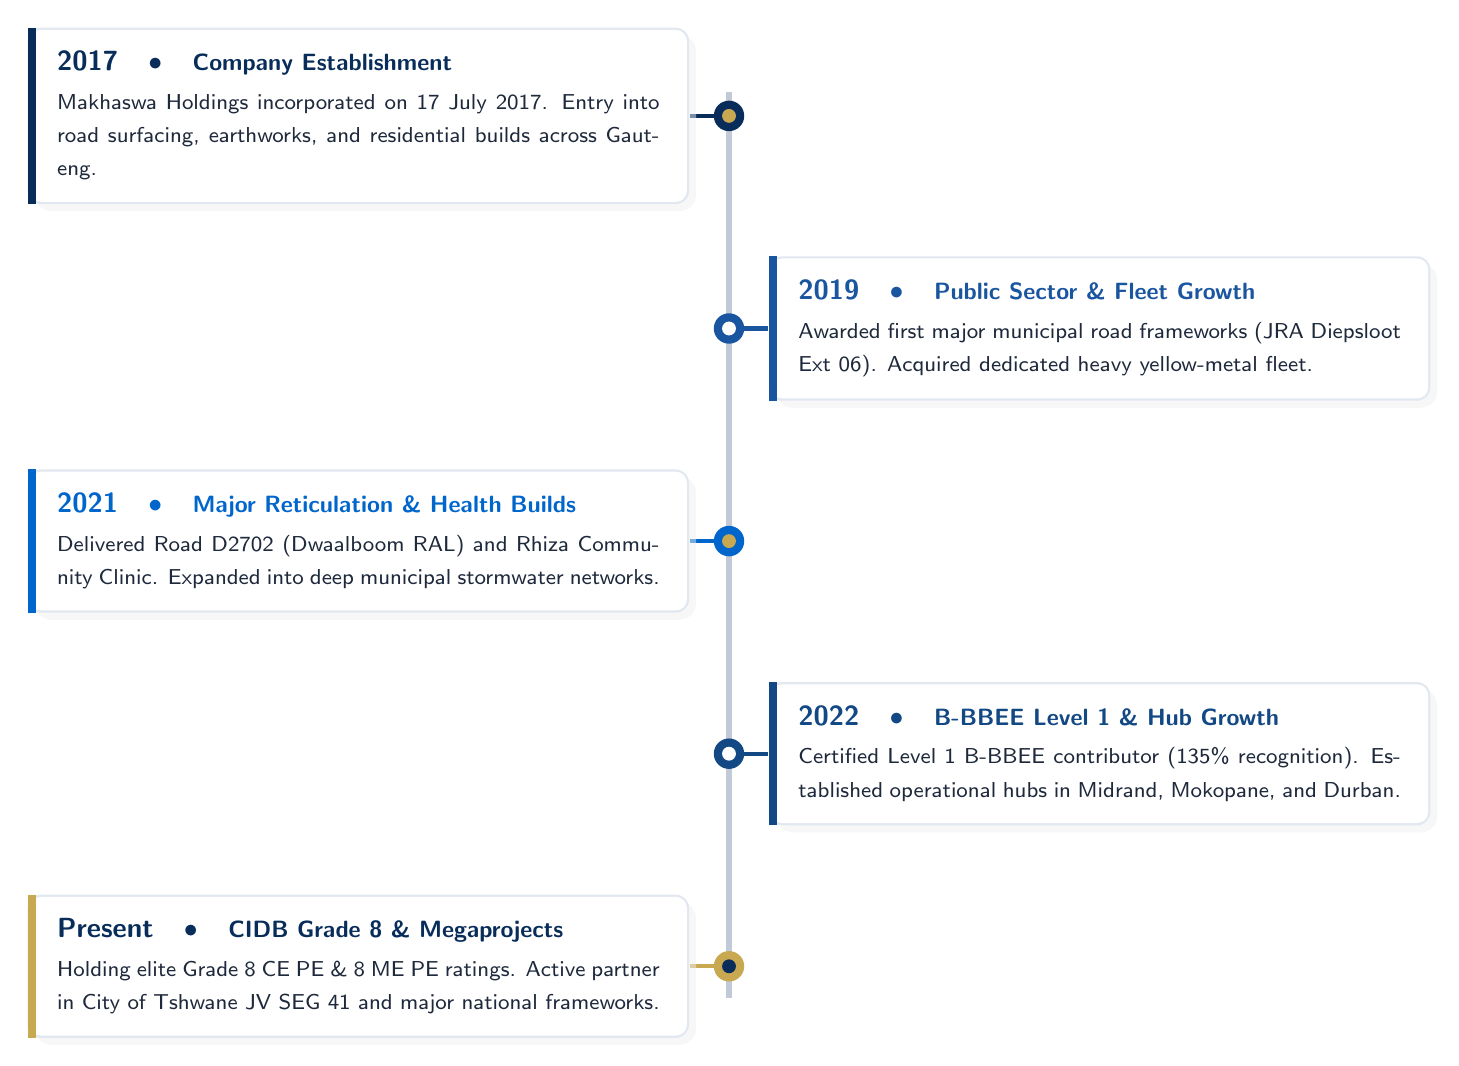
\begin{tikzpicture}[x=1cm, y=1cm]
    % Central Spine Line
    \draw[color=mhnavy!25, line width=2pt] (0, 0.3) -- (0, -11.2);

    % ----------------------------------------------------
    % 2017 --- LEFT SIDE (Company Establishment)
    % ----------------------------------------------------
    \draw[color=mhnavy, line width=1.5pt] (-0.5, 0.0) -- (0, 0.0);
    \fill[mhnavy] (0, 0.0) circle (5.5pt);
    \fill[mhgold] (0, 0.0) circle (2.5pt);
    \node[anchor=east, inner sep=0pt] at (-0.5, 0.0) {
        \begin{minipage}{8.4cm}
            \begin{tcolorbox}[
                enhanced, colback=white, colframe=mhlightgray, boxrule=0.8pt, arc=4pt,
                left=7pt, right=7pt, top=5pt, bottom=5pt,
                borderline west={3pt}{0pt}{mhnavy}, drop shadow=black!6
            ]
                {\fontsize{10pt}{12pt}\selectfont\bfseries\color{mhnavy}2017 \ \ $\bullet$ \ \ \fontsize{8.5pt}{10pt}\selectfont Company Establishment}\\[2pt]
                {\fontsize{7.8pt}{10.5pt}\selectfont\color{mhtext}Makhaswa Holdings incorporated on 17 July 2017. Entry into road surfacing, earthworks, and residential builds across Gauteng.}
            \end{tcolorbox}
        \end{minipage}
    };

    % ----------------------------------------------------
    % 2019 --- RIGHT SIDE (Public Sector & Fleet Expansion)
    % ----------------------------------------------------
    \draw[color=mhblue, line width=1.5pt] (0, -2.7) -- (0.5, -2.7);
    \fill[mhblue] (0, -2.7) circle (5.5pt);
    \fill[white] (0, -2.7) circle (2.5pt);
    \node[anchor=west, inner sep=0pt] at (0.5, -2.7) {
        \begin{minipage}{8.4cm}
            \begin{tcolorbox}[
                enhanced, colback=white, colframe=mhlightgray, boxrule=0.8pt, arc=4pt,
                left=7pt, right=7pt, top=5pt, bottom=5pt,
                borderline west={3pt}{0pt}{mhblue}, drop shadow=black!6
            ]
                {\fontsize{10pt}{12pt}\selectfont\bfseries\color{mhblue}2019 \ \ $\bullet$ \ \ \fontsize{8.5pt}{10pt}\selectfont Public Sector \& Fleet Growth}\\[2pt]
                {\fontsize{7.8pt}{10.5pt}\selectfont\color{mhtext}Awarded first major municipal road frameworks (JRA Diepsloot Ext 06). Acquired dedicated heavy yellow-metal fleet.}
            \end{tcolorbox}
        \end{minipage}
    };

    % ----------------------------------------------------
    % 2021 --- LEFT SIDE (Major Reticulation & Healthcare)
    % ----------------------------------------------------
    \draw[color=mhbluebright, line width=1.5pt] (-0.5, -5.4) -- (0, -5.4);
    \fill[mhbluebright] (0, -5.4) circle (5.5pt);
    \fill[mhgold] (0, -5.4) circle (2.5pt);
    \node[anchor=east, inner sep=0pt] at (-0.5, -5.4) {
        \begin{minipage}{8.4cm}
            \begin{tcolorbox}[
                enhanced, colback=white, colframe=mhlightgray, boxrule=0.8pt, arc=4pt,
                left=7pt, right=7pt, top=5pt, bottom=5pt,
                borderline west={3pt}{0pt}{mhbluebright}, drop shadow=black!6
            ]
                {\fontsize{10pt}{12pt}\selectfont\bfseries\color{mhbluebright}2021 \ \ $\bullet$ \ \ \fontsize{8.5pt}{10pt}\selectfont Major Reticulation \& Health Builds}\\[2pt]
                {\fontsize{7.8pt}{10.5pt}\selectfont\color{mhtext}Delivered Road D2702 (Dwaalboom RAL) and Rhiza Community Clinic. Expanded into deep municipal stormwater networks.}
            \end{tcolorbox}
        \end{minipage}
    };

    % ----------------------------------------------------
    % 2022 --- RIGHT SIDE (B-BBEE Level 1 & Multi-Hubs)
    % ----------------------------------------------------
    \draw[color=mhnavy3, line width=1.5pt] (0, -8.1) -- (0.5, -8.1);
    \fill[mhnavy3] (0, -8.1) circle (5.5pt);
    \fill[white] (0, -8.1) circle (2.5pt);
    \node[anchor=west, inner sep=0pt] at (0.5, -8.1) {
        \begin{minipage}{8.4cm}
            \begin{tcolorbox}[
                enhanced, colback=white, colframe=mhlightgray, boxrule=0.8pt, arc=4pt,
                left=7pt, right=7pt, top=5pt, bottom=5pt,
                borderline west={3pt}{0pt}{mhnavy3}, drop shadow=black!6
            ]
                {\fontsize{10pt}{12pt}\selectfont\bfseries\color{mhnavy3}2022 \ \ $\bullet$ \ \ \fontsize{8.5pt}{10pt}\selectfont B-BBEE Level 1 \& Hub Growth}\\[2pt]
                {\fontsize{7.8pt}{10.5pt}\selectfont\color{mhtext}Certified Level 1 B-BBEE contributor (135\% recognition). Established operational hubs in Midrand, Mokopane, and Durban.}
            \end{tcolorbox}
        \end{minipage}
    };

    % ----------------------------------------------------
    % PRESENT --- LEFT SIDE (CIDB Grade 8 & Megaprojects)
    % ----------------------------------------------------
    \draw[color=mhgold, line width=1.5pt] (-0.5, -10.8) -- (0, -10.8);
    \fill[mhgold] (0, -10.8) circle (5.5pt);
    \fill[mhnavy] (0, -10.8) circle (2.5pt);
    \node[anchor=east, inner sep=0pt] at (-0.5, -10.8) {
        \begin{minipage}{8.4cm}
            \begin{tcolorbox}[
                enhanced, colback=white, colframe=mhlightgray, boxrule=0.8pt, arc=4pt,
                left=7pt, right=7pt, top=5pt, bottom=5pt,
                borderline west={3pt}{0pt}{mhgold}, drop shadow=black!6
            ]
                {\fontsize{10pt}{12pt}\selectfont\bfseries\color{mhnavy}Present \ \ $\bullet$ \ \ \fontsize{8.5pt}{10pt}\selectfont CIDB Grade 8 \& Megaprojects}\\[2pt]
                {\fontsize{7.8pt}{10.5pt}\selectfont\color{mhtext}Holding elite Grade 8 CE PE \& 8 ME PE ratings. Active partner in City of Tshwane JV SEG 41 and major national frameworks.}
            \end{tcolorbox}
        \end{minipage}
    };
\end{tikzpicture}
\end{center}

\vspace{0.1cm}

% Bottom Milestone Stats Strip
\noindent
\begin{minipage}[t]{0.235\textwidth}\statcard{mhnavy}{2017}{Year Established}\end{minipage}\hfill
\begin{minipage}[t]{0.235\textwidth}\statcard{mhblue}{Grade 8}{CE PE / 8 ME PE}\end{minipage}\hfill
\begin{minipage}[t]{0.235\textwidth}\statcard{mhbluebright}{Level 1}{B-BBEE Contributor}\end{minipage}\hfill
\begin{minipage}[t]{0.235\textwidth}\statcard{mhnavy3}{100\%}{Black-Owned Firm}\end{minipage}

\clearpage

% =================================================
% PAGE 8 (CONTENT p.5) --- CORE ENGINEERING DISCIPLINES & CAPABILITIES
% =================================================

\sectionbanner{OUR SERVICES}{Core Engineering Disciplines \& Technical Capabilities}

\noindent
\begin{minipage}[t]{0.485\textwidth}
    \servicecard{01. Bulk Earthworks \& Ground Engineering}{Clearing, 300mm topsoil stripping, cut-to-fill balancing, mass terrace preparation, basement excavation, subgrade ripping to 90\%--93\% Mod AASHTO, lime/cement stabilization, and dump rock filling for wet ground.}
    \vspace{0.18cm}
    \servicecard{02. Road Construction, Layerworks \& Surfacing}{Imported dump rock subgrade, selected G7/G5, stabilized C3/C4 sub-base, and G1/G2 base compacted to 98\%--102\% Mod AASHTO. Continuous-graded asphalt, slurry seals, chip-and-spray, and 60mm/80mm Type SA paving.}
    \vspace{0.18cm}
    \servicecard{03. Civil Stormwater \& Drainage Infrastructure}{Supply and laying of 450mm--1200mm spigot and socket concrete pipes, Class 100D Ogee pipes, portal box culverts, in-situ concrete/brick manholes, JRA kerb inlets (JRA-SD-SW-020--024), and 110mm Kaytech subsoil pipes.}
\end{minipage}
\hfill
\begin{minipage}[t]{0.485\textwidth}
    \servicecard{04. Potable Water \& Gravity Sewer Reticulation}{Excavation, bedding, laying of uPVC, mPVC, HDPE, and ductile iron pipelines, pressure testing, disinfection, individual erf meter connections, gravity sewer outfalls, pump stations, and reservoirs.}
    \vspace{0.18cm}
    \servicecard{05. General Building \& Structural Facilities}{NHBRC Class 5 registered builder. Turnkey delivery of commercial office parks, municipal depots, health clinics, school classroom blocks, ablution facilities, and residential estates from foundations to final finishes.}
    \vspace{0.18cm}
    \servicecard{06. Electrical Reticulation \& High-Mast Lighting}{Excavation and casting of structural plinths, high-mast lighting pole erection, luminaire mounting, cabling, LV/MV reticulation, and perimeter security fencing (palisade and weldmesh).}
\end{minipage}

\vspace{0.25cm}

% Discipline Images Strip
\noindent
\begin{minipage}[t]{0.235\textwidth}
    \begin{tcolorbox}[enhanced, colback=white, colframe=mhlightgray, boxrule=0.6pt, arc=3pt, left=0pt, right=0pt, top=0pt, bottom=3pt]
        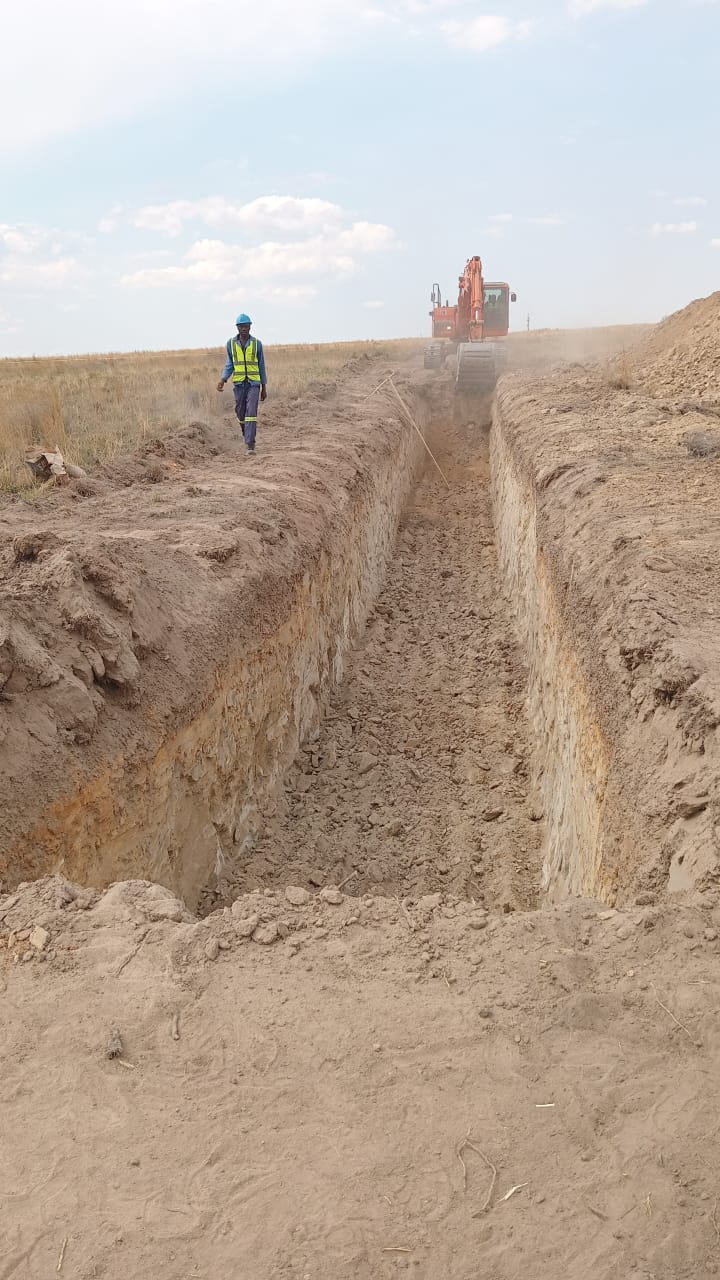
\includegraphics[width=\linewidth, height=2.2cm, keepaspectratio=false]{images/bulk-trenching-earthworks-1.jpeg}
        \centering\vspace{2pt}
        {\fontsize{7.2pt}{8.5pt}\selectfont\bfseries\color{mhnavy}Bulk Earthworks}
    \end{tcolorbox}
\end{minipage}\hfill
\begin{minipage}[t]{0.235\textwidth}
    \begin{tcolorbox}[enhanced, colback=white, colframe=mhlightgray, boxrule=0.6pt, arc=3pt, left=0pt, right=0pt, top=0pt, bottom=3pt]
        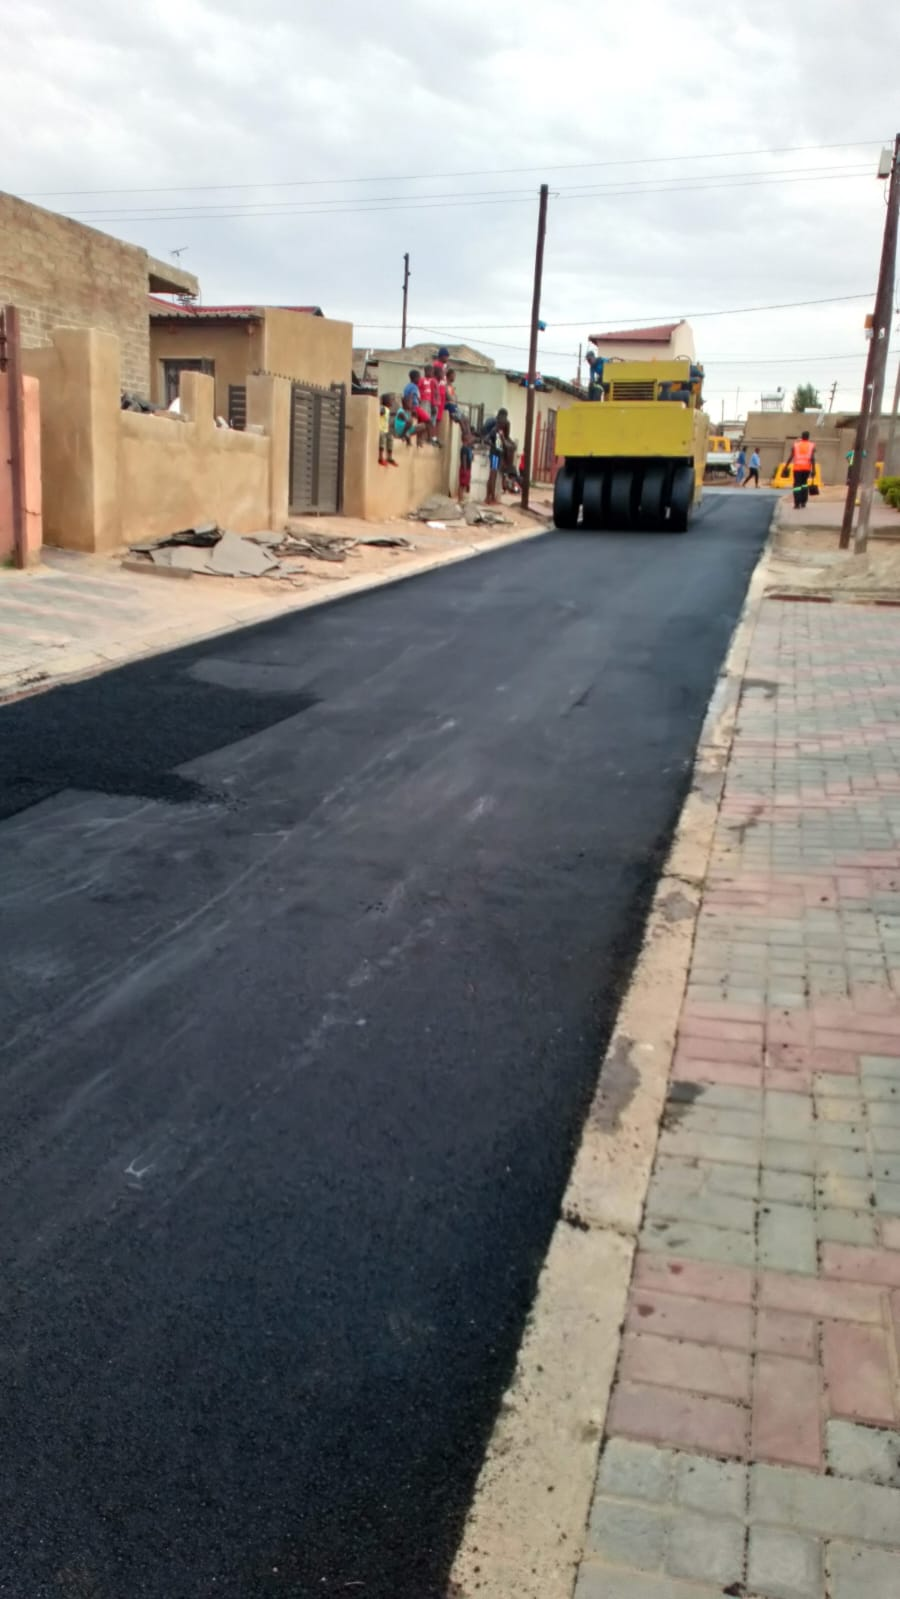
\includegraphics[width=\linewidth, height=2.2cm, keepaspectratio=false]{images/asphalt-photos-1.jpeg}
        \centering\vspace{2pt}
        {\fontsize{7.2pt}{8.5pt}\selectfont\bfseries\color{mhnavy}Roads \& Layerworks}
    \end{tcolorbox}
\end{minipage}\hfill
\begin{minipage}[t]{0.235\textwidth}
    \begin{tcolorbox}[enhanced, colback=white, colframe=mhlightgray, boxrule=0.6pt, arc=3pt, left=0pt, right=0pt, top=0pt, bottom=3pt]
        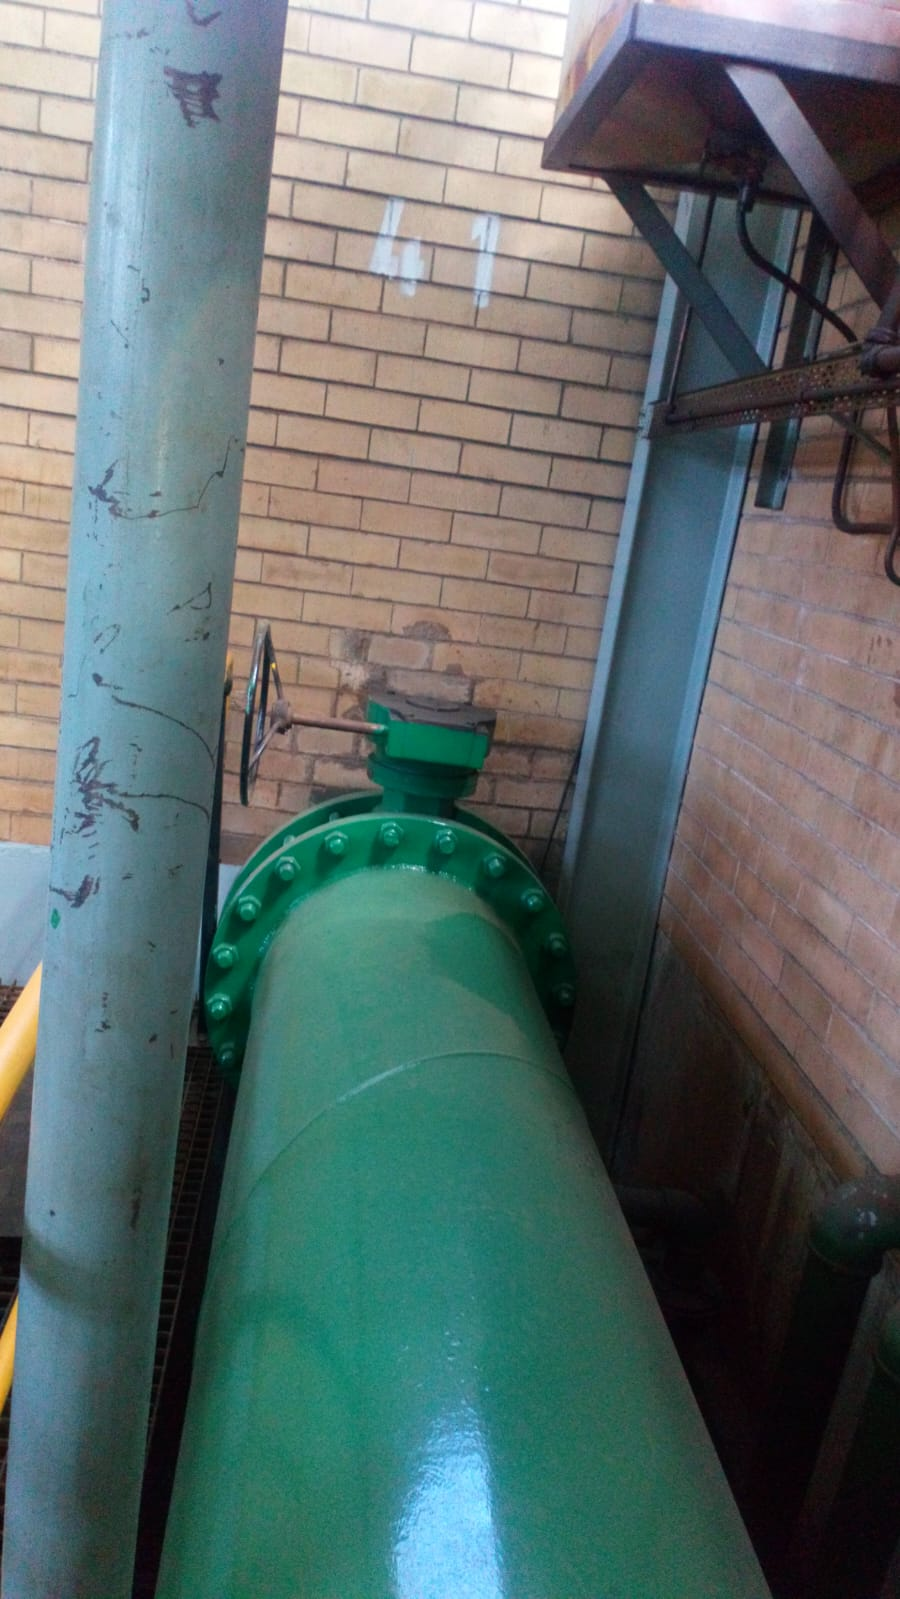
\includegraphics[width=\linewidth, height=2.2cm, keepaspectratio=false]{images/pumphouse-steel-pipe-works-1.jpeg}
        \centering\vspace{2pt}
        {\fontsize{7.2pt}{8.5pt}\selectfont\bfseries\color{mhnavy}Water Reticulation}
    \end{tcolorbox}
\end{minipage}\hfill
\begin{minipage}[t]{0.235\textwidth}
    \begin{tcolorbox}[enhanced, colback=white, colframe=mhlightgray, boxrule=0.6pt, arc=3pt, left=0pt, right=0pt, top=0pt, bottom=3pt]
        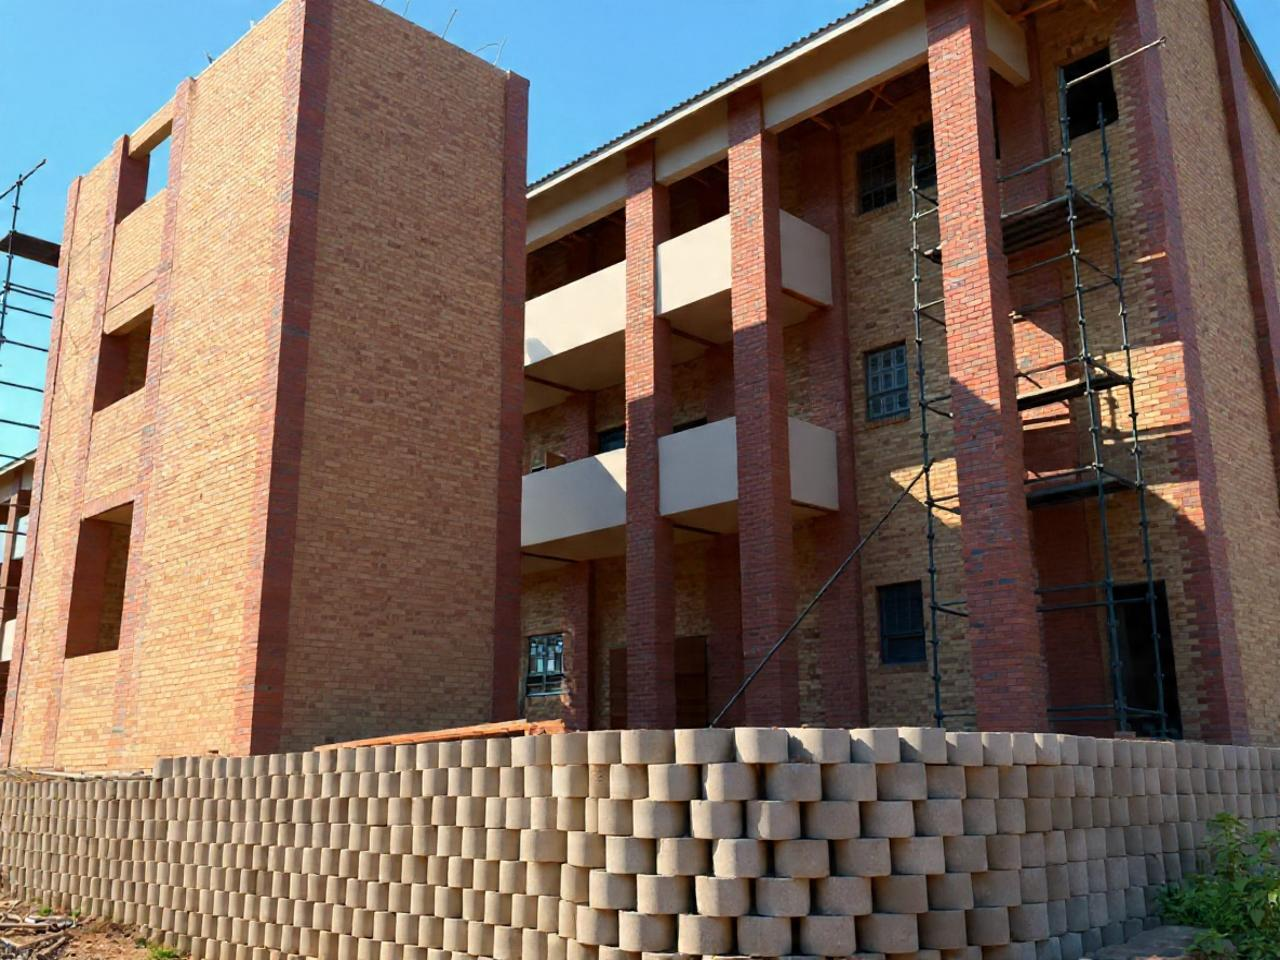
\includegraphics[width=\linewidth, height=2.2cm, keepaspectratio=false]{images/building-construction-commercial.jpeg}
        \centering\vspace{2pt}
        {\fontsize{7.2pt}{8.5pt}\selectfont\bfseries\color{mhnavy}General Building}
    \end{tcolorbox}
\end{minipage}

\vspace{0.25cm}

{\large\bfseries\color{mhnavy} Five-Stage Project Delivery Methodology}
\vspace{0.15cm}

\noindent
\begin{minipage}[t]{0.185\textwidth}\statcard{mhnavy}{01}{Planning}\end{minipage}\hfill
\begin{minipage}[t]{0.185\textwidth}\statcard{mhblue}{02}{Procurement}\end{minipage}\hfill
\begin{minipage}[t]{0.185\textwidth}\statcard{mhbluebright}{03}{Execution}\end{minipage}\hfill
\begin{minipage}[t]{0.185\textwidth}\statcard{mhnavy3}{04}{QA / QC}\end{minipage}\hfill
\begin{minipage}[t]{0.185\textwidth}\statcard{mhblue}{05}{Handover}\end{minipage}

\clearpage

% =================================================
% PAGE 9 (CONTENT p.6) --- PLANT, FLEET & OPERATIONAL CAPACITY
% =================================================

\sectionbanner{OPERATIONAL CAPACITY}{Plant, Fleet, Equipment \& Technical Software}

\noindent
{\fontsize{9pt}{12.8pt}\selectfont\color{mhtext}
Makhaswa Holdings manages a comprehensive plant fleet, transport logistics, and precision survey instrumentation through company-owned machinery and preferred commercial plant-hire partnerships, ensuring rapid mobilization:
}

\vspace{0.25cm}

\renewcommand{\arraystretch}{1.22}
\begin{tabularx}{\textwidth}{@{}p{4.2cm} p{2.5cm} X@{}}
\rowcolor{mhnavy}
{\color{white}\bfseries\fontsize{8pt}{10pt}\selectfont Machinery Category} & {\color{white}\bfseries\fontsize{8pt}{10pt}\selectfont Operational Status} & {\color{white}\bfseries\fontsize{8pt}{10pt}\selectfont Specified Fleet \& Instrumentation Capacity} \\
\rowcolor{mhbluelight}
\fontsize{7.8pt}{9.5pt}\selectfont\bfseries Earthmoving \& Excavation & \fontsize{7.8pt}{9.5pt}\selectfont Core Fleet / Hired & \fontsize{7.8pt}{9.5pt}\selectfont 20t--30t Tracked Excavators, 4x4 Heavy TLBs, 140K/140H Motor Graders, D6/D7 Dozers \\
\fontsize{7.8pt}{9.5pt}\selectfont\bfseries Compaction \& Surfacing & \fontsize{7.8pt}{9.5pt}\selectfont Core Fleet / Hired & \fontsize{7.8pt}{9.5pt}\selectfont 10t--12t Smooth-Drum Rollers, Padfoot Compactors, Bitumen Asphalt Pavers, Walk-behind Rollers \\
\rowcolor{mhbluelight}
\fontsize{7.8pt}{9.5pt}\selectfont\bfseries Haulage \& Logistics & \fontsize{7.8pt}{9.5pt}\selectfont Core Fleet / Hired & \fontsize{7.8pt}{9.5pt}\selectfont 10m$^3$--15m$^3$ Tipper Trucks, 30t Low-Bed Horses \& Trailers, 10,000L--16,000L Water Tankers \\
\fontsize{7.8pt}{9.5pt}\selectfont\bfseries Survey \& Testing Instruments & \fontsize{7.8pt}{9.5pt}\selectfont Company-Owned & \fontsize{7.8pt}{9.5pt}\selectfont Leica/Topcon Total Stations, RTK Dual-Frequency GPS, Troxler Gauges, Slump \& Cube Kits \\
\rowcolor{mhbluelight}
\fontsize{7.8pt}{9.5pt}\selectfont\bfseries Site Utilities \& Power & \fontsize{7.8pt}{9.5pt}\selectfont Company-Owned & \fontsize{7.8pt}{9.5pt}\selectfont 50kVA--150kVA Mobile Generators, High-pressure Air Compressors, Mobile Site Offices \& Ablutions \\
\fontsize{7.8pt}{9.5pt}\selectfont\bfseries Technical \& Project Software & \fontsize{7.8pt}{9.5pt}\selectfont Licensed & \fontsize{7.8pt}{9.5pt}\selectfont AutoCAD 2024, AutoCAD Civil 3D, MS Project, Primavera P6, Model Maker, CCS Candy \& WinQS \\
\end{tabularx}
\renewcommand{\arraystretch}{1}

\vspace{0.3cm}

% Fleet in Action Showcase
\noindent
\begin{minipage}[t]{0.315\textwidth}
    \begin{tcolorbox}[enhanced, colback=white, colframe=mhlightgray, boxrule=0.7pt, arc=3pt, left=0pt, right=0pt, top=0pt, bottom=3pt]
        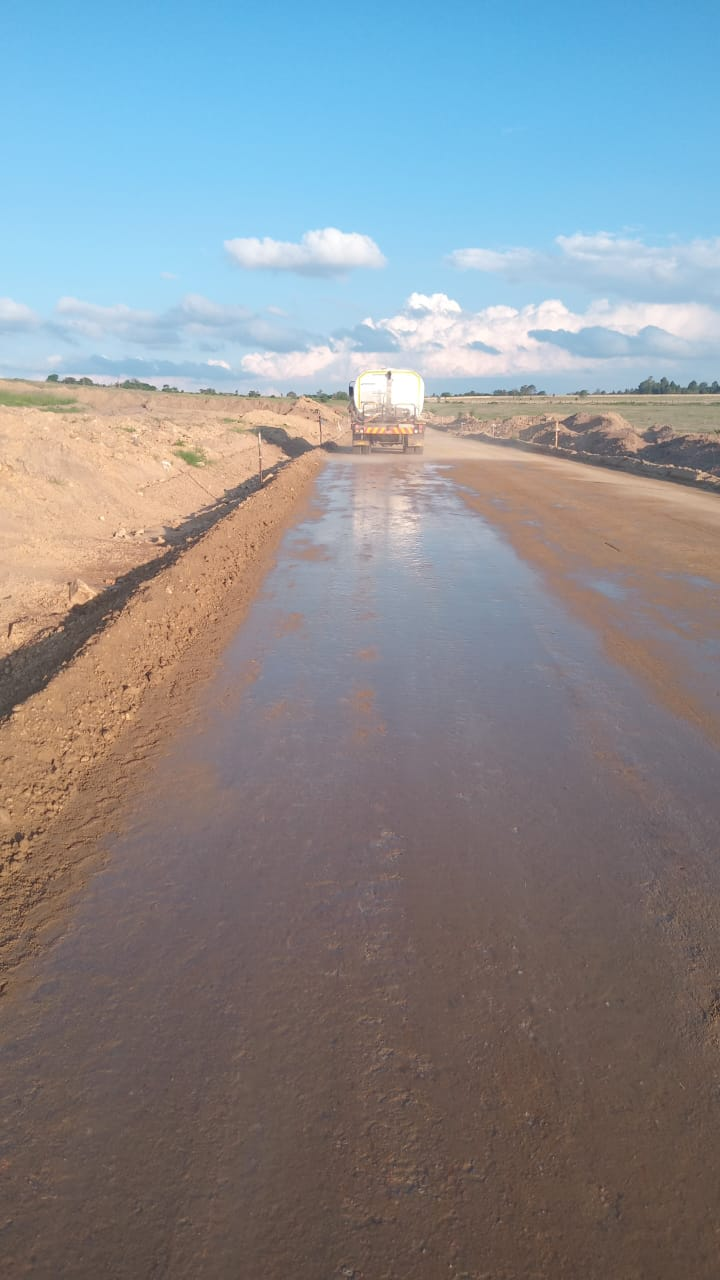
\includegraphics[width=\linewidth, height=2.6cm, keepaspectratio=false]{images/earthworks-surfacing-watertruck.jpeg}
        \centering\vspace{2pt}
        {\fontsize{7.2pt}{8.5pt}\selectfont\bfseries\color{mhnavy}Yellow Metal \& Water Tankers}
    \end{tcolorbox}
\end{minipage}\hfill
\begin{minipage}[t]{0.315\textwidth}
    \begin{tcolorbox}[enhanced, colback=white, colframe=mhlightgray, boxrule=0.7pt, arc=3pt, left=0pt, right=0pt, top=0pt, bottom=3pt]
        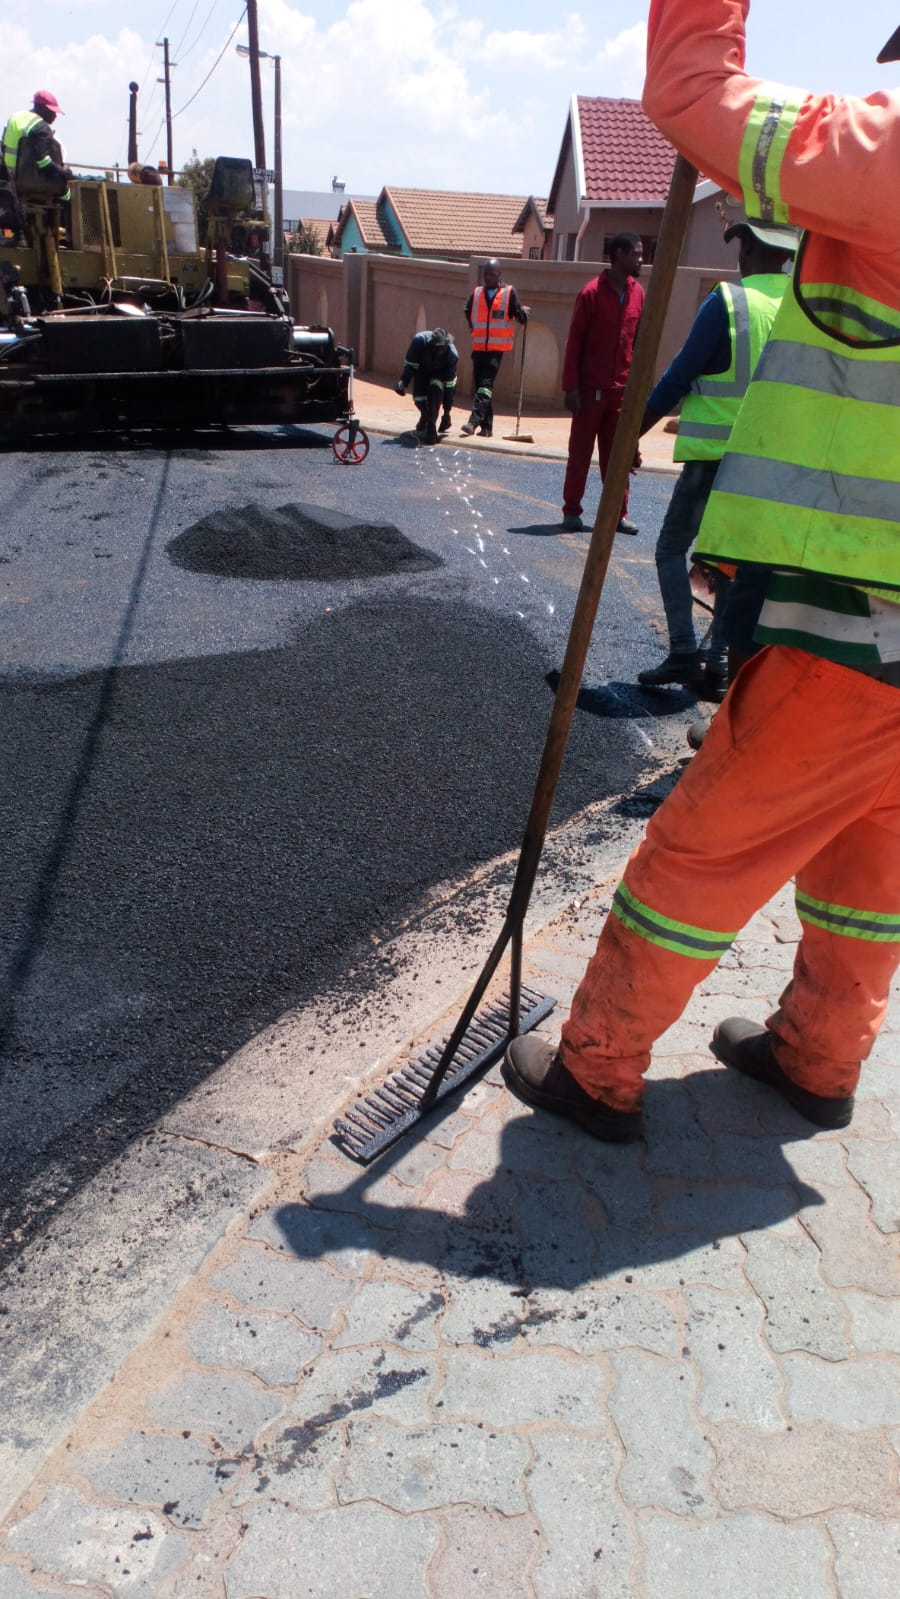
\includegraphics[width=\linewidth, height=2.6cm, keepaspectratio=false]{images/asphalt-photos-2.jpeg}
        \centering\vspace{2pt}
        {\fontsize{7.2pt}{8.5pt}\selectfont\bfseries\color{mhnavy}Asphalt Pavers \& Surfacing Fleet}
    \end{tcolorbox}
\end{minipage}\hfill
\begin{minipage}[t]{0.315\textwidth}
    \begin{tcolorbox}[enhanced, colback=white, colframe=mhlightgray, boxrule=0.7pt, arc=3pt, left=0pt, right=0pt, top=0pt, bottom=3pt]
        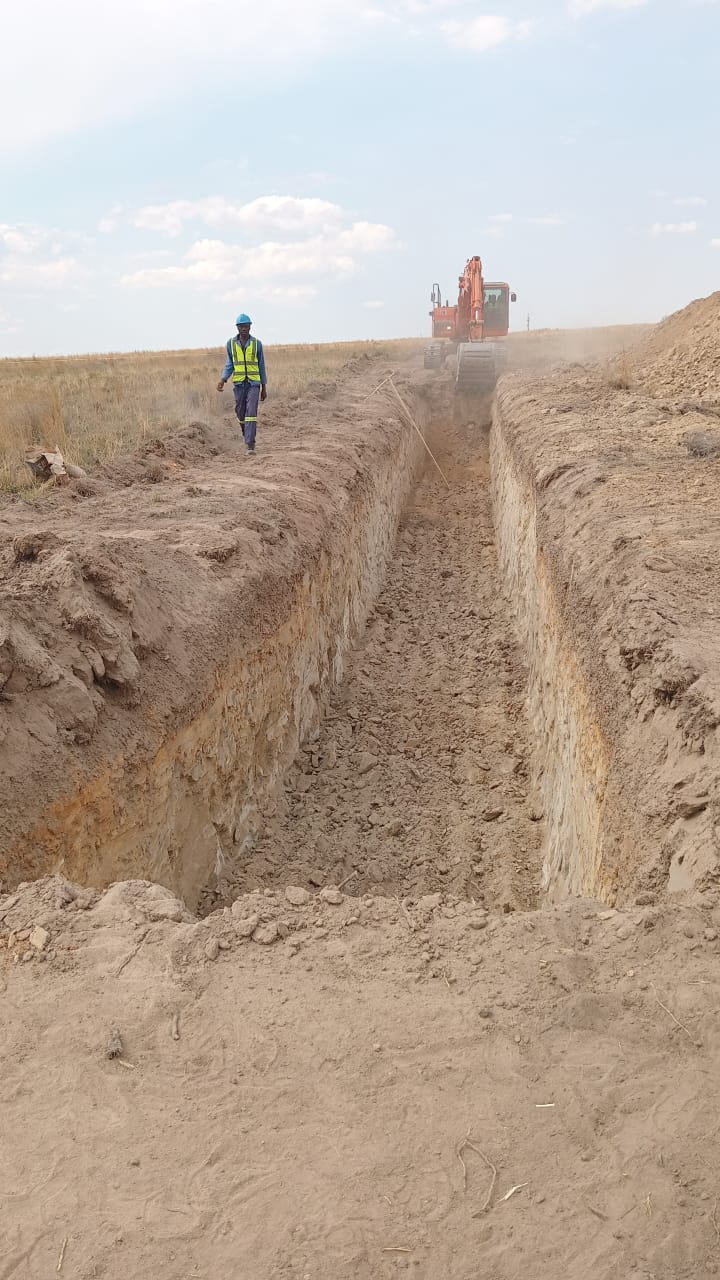
\includegraphics[width=\linewidth, height=2.6cm, keepaspectratio=false]{images/bulk-trenching-earthworks-1.jpeg}
        \centering\vspace{2pt}
        {\fontsize{7.2pt}{8.5pt}\selectfont\bfseries\color{mhnavy}Heavy Trenching \& Excavators}
    \end{tcolorbox}
\end{minipage}

\vspace{0.3cm}

\noindent
\begin{minipage}[t]{0.315\textwidth}\statcard{mhnavy}{Multi-Fleet}{Deployment Logistics}\end{minipage}\hfill
\begin{minipage}[t]{0.315\textwidth}\statcard{mhblue}{Pr.Eng / OHS}{Site Supervisory Control}\end{minipage}\hfill
\begin{minipage}[t]{0.315\textwidth}\statcard{mhbluebright}{Multi-Site}{Concurrent Deployments}\end{minipage}

\clearpage

% =================================================
% PAGE 10 (CONTENT p.7) --- SHEQ POLICY, ISO ALIGNMENT & LAB TESTING
% =================================================

\sectionbanner{SHEQ FRAMEWORK}{Safety, Health, Environment \& Quality Governance}

\noindent
\begin{minipage}[t]{0.31\textwidth}
    \begin{tcolorbox}[
        enhanced, colback=white, colframe=mhlightgray, boxrule=0.8pt, arc=4pt,
        title={\bfseries\color{white} Occupational Health \& Safety},
        colbacktitle=mhnavy, fonttitle=\bfseries\small,
        left=8pt, right=8pt, top=8pt, bottom=8pt, height=6.0cm
    ]
        {\fontsize{8pt}{11pt}\selectfont\color{mhtext}
        \textbf{Zero Harm Commitment:} Strict adherence to the OHS Act (Act 85 of 1993) and Construction Regulations 2014. Mandatory daily toolbox talks, SABS-approved PPE enforcement, appointed SHEQ Officers (Pr.OHS), continuous hazard logs, and full OHS site compliance.
        }
    \end{tcolorbox}
\end{minipage}
\hfill
\begin{minipage}[t]{0.31\textwidth}
    \begin{tcolorbox}[
        enhanced, colback=white, colframe=mhlightgray, boxrule=0.8pt, arc=4pt,
        title={\bfseries\color{white} Quality Assurance \& Testing},
        colbacktitle=mhblue, fonttitle=\bfseries\small,
        left=8pt, right=8pt, top=8pt, bottom=8pt, height=6.0cm
    ]
        {\fontsize{8pt}{11pt}\selectfont\color{mhtext}
        \textbf{ISO 9001:2015 Alignment:} Documented Inspection and Test Plans (ITPs). Compaction verification via Troxler nuclear density gauges, concrete slump testing, and 150mm cube sampling with 7-, 14-, and 28-day compression crushing at SANAS-accredited testing laboratories.
        }
    \end{tcolorbox}
\end{minipage}
\hfill
\begin{minipage}[t]{0.31\textwidth}
    \begin{tcolorbox}[
        enhanced, colback=white, colframe=mhlightgray, boxrule=0.8pt, arc=4pt,
        title={\bfseries\color{white} Environmental Management},
        colbacktitle=mhbluebright, fonttitle=\bfseries\small,
        left=8pt, right=8pt, top=8pt, bottom=8pt, height=6.0cm
    ]
        {\fontsize{8pt}{11pt}\selectfont\color{mhtext}
        \textbf{ISO 14001:2015 Alignment:} Proactive silt trapping, runoff control berms, bunded hazardous fuel/chemical storage areas, certified waste disposal, topsoil stripping and stockpiling for complete post-construction landscape rehabilitation.
        }
    \end{tcolorbox}
\end{minipage}

\vspace{0.35cm}

% SHEQ Visual Accents
\noindent
\begin{minipage}[t]{0.485\textwidth}
    \begin{tcolorbox}[enhanced, colback=mhoffwhite, colframe=mhlightgray, boxrule=0.7pt, arc=4pt, left=8pt, right=8pt, top=6pt, bottom=6pt]
        \begin{minipage}[c]{0.3\textwidth}
            
\includegraphics[width=\linewidth, height=1.4cm, keepaspectratio]{images/sheq-logo.png}
        \end{minipage}\hfill
        \begin{minipage}[c]{0.65\textwidth}
            {\fontsize{8.5pt}{11pt}\selectfont\bfseries\color{mhnavy}Integrated SHEQ Protocols}\\[2pt]
            {\fontsize{7.5pt}{9.8pt}\selectfont\color{mhtextmuted}Daily safety checks, risk logs, and complete site compliance auditing.}
        \end{minipage}
    \end{tcolorbox}
\end{minipage}\hfill
\begin{minipage}[t]{0.485\textwidth}
    \begin{tcolorbox}[enhanced, colback=mhoffwhite, colframe=mhlightgray, boxrule=0.7pt, arc=4pt, left=8pt, right=8pt, top=6pt, bottom=6pt]
        \begin{minipage}[c]{0.3\textwidth}
            
\includegraphics[width=\linewidth, height=1.4cm, keepaspectratio]{images/iso-logo.png}
        \end{minipage}\hfill
        \begin{minipage}[c]{0.65\textwidth}
            {\fontsize{8.5pt}{11pt}\selectfont\bfseries\color{mhnavy}ISO System Framework Alignment}\\[2pt]
            {\fontsize{7.5pt}{9.8pt}\selectfont\color{mhtextmuted}ISO 9001 (Quality), ISO 14001 (Environment), ISO 45001 (OH\&S).}
        \end{minipage}
    \end{tcolorbox}
\end{minipage}

\vspace{0.35cm}

{\large\bfseries\color{mhnavy} Our SHEQ Commitment in Numbers}
\vspace{0.15cm}

\noindent
\begin{minipage}[t]{0.235\textwidth}\statcard{mhnavy}{ISO Standards}{9001 $\bullet$ 14001 $\bullet$ 45001}\end{minipage}\hfill
\begin{minipage}[t]{0.235\textwidth}\statcard{mhblue}{Zero Harm}{Safety Target}\end{minipage}\hfill
\begin{minipage}[t]{0.235\textwidth}\statcard{mhbluebright}{OHS Act}{85 of 1993 Compliant}\end{minipage}\hfill
\begin{minipage}[t]{0.235\textwidth}\statcard{mhnavy3}{Daily}{Toolbox Talks}\end{minipage}

\clearpage

% =================================================
% PAGE 11 (CONTENT p.8) --- FLAGSHIP PROJECT PORTFOLIO: CIVIL INFRASTRUCTURE & ROADS
% =================================================

\sectionbanner{PROJECT PORTFOLIO}{Civil Infrastructure, Roads \& Stormwater Schemes}

\noindent
\begin{minipage}[t]{0.235\textwidth}
    \begin{tcolorbox}[enhanced, colback=white, colframe=mhlightgray, boxrule=0.7pt, arc=3pt, left=0pt, right=0pt, top=0pt, bottom=3pt]
        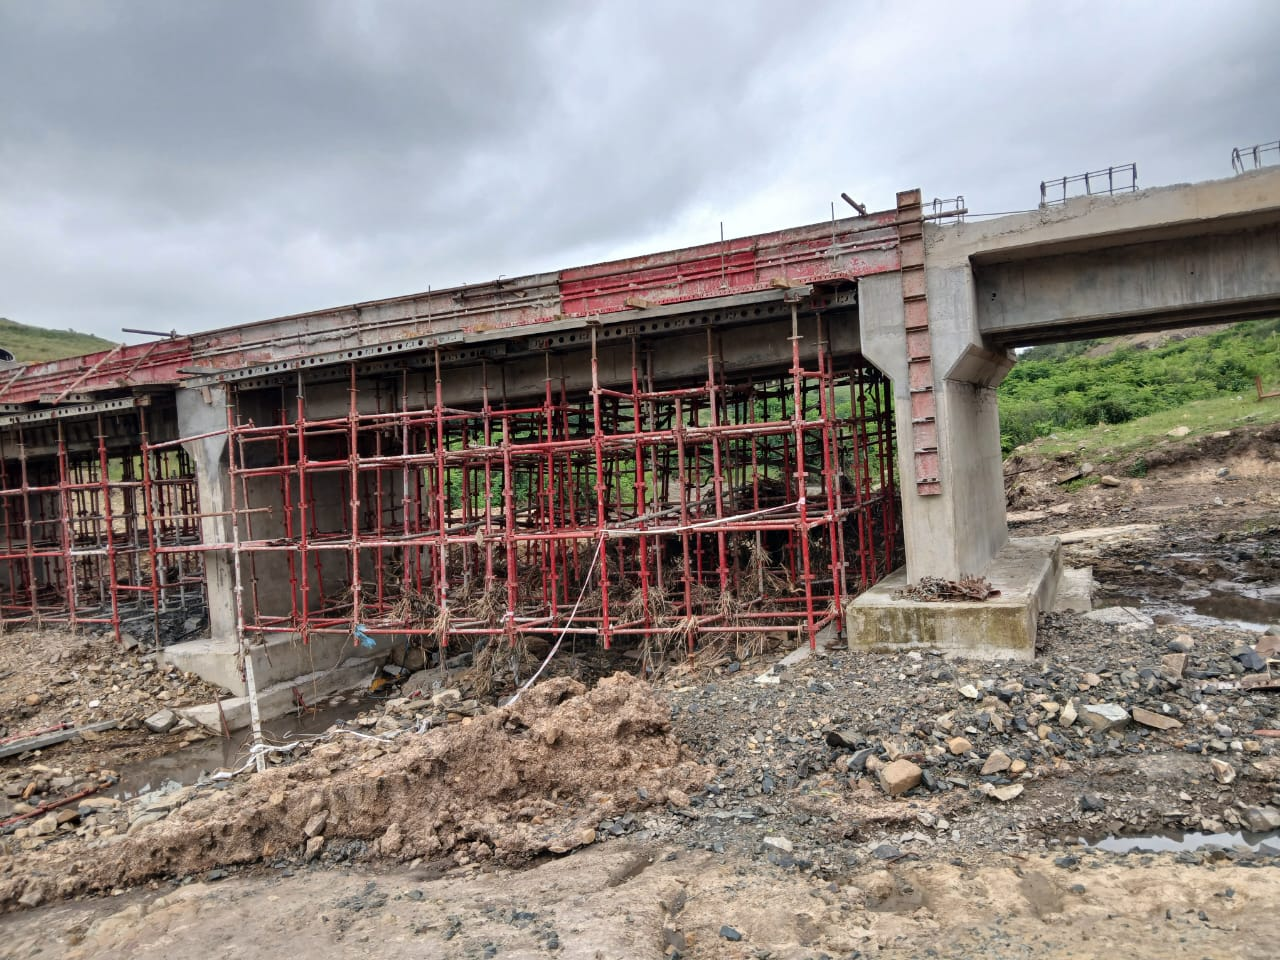
\includegraphics[width=\linewidth, height=2.4cm, keepaspectratio=false]{images/concrete-bridges-1.jpeg}
        \centering\vspace{2pt}
        {\fontsize{7pt}{8pt}\selectfont\bfseries\color{mhtextmuted}CIVIL INFRASTRUCTURE}\\[1pt]
        {\fontsize{7.5pt}{9pt}\selectfont\bfseries\color{mhnavy}Concrete Bridges \& Culverts}
    \end{tcolorbox}
\end{minipage}\hfill
\begin{minipage}[t]{0.235\textwidth}
    \begin{tcolorbox}[enhanced, colback=white, colframe=mhlightgray, boxrule=0.7pt, arc=3pt, left=0pt, right=0pt, top=0pt, bottom=3pt]
        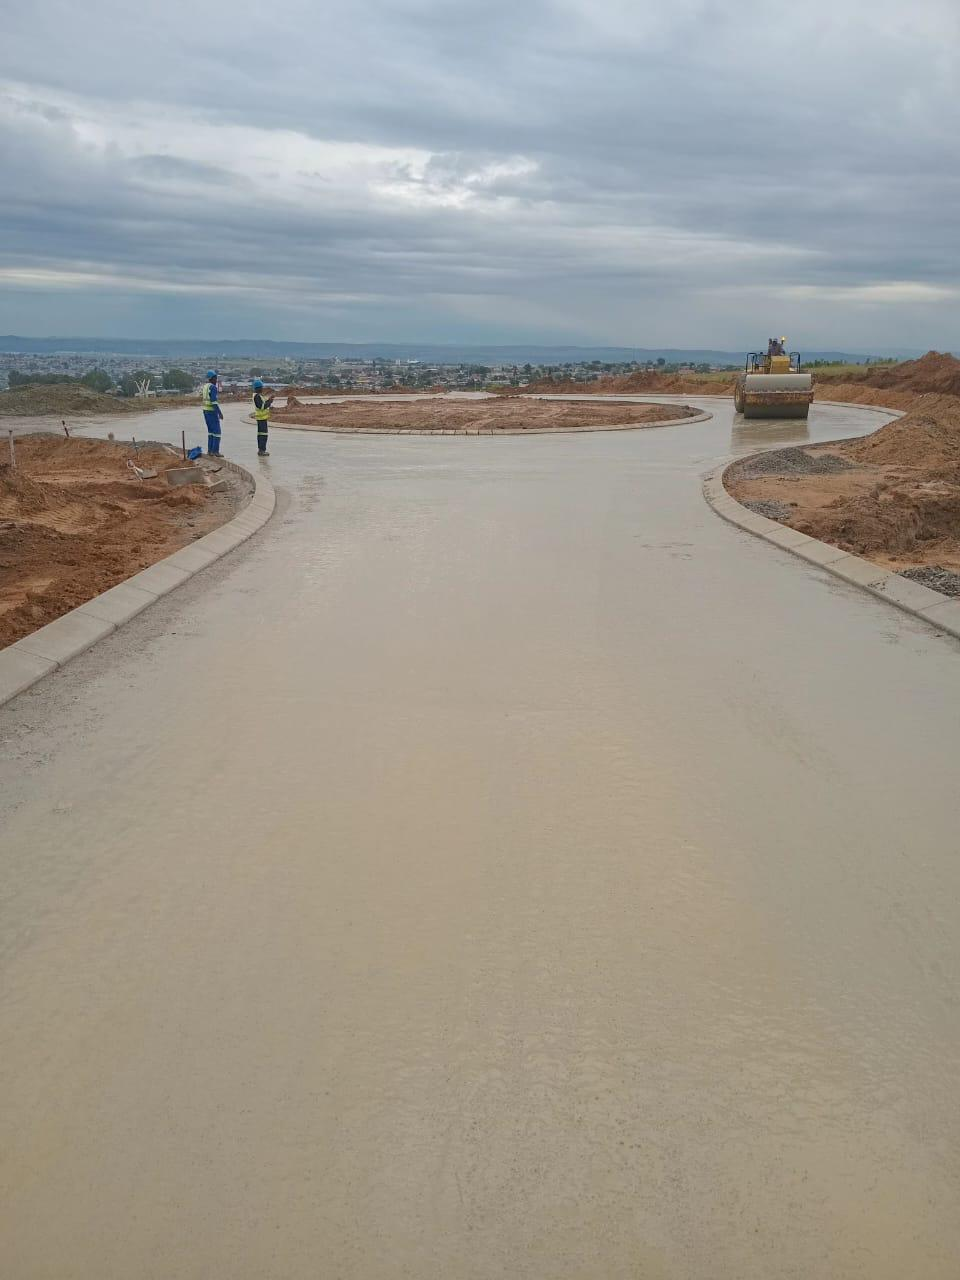
\includegraphics[width=\linewidth, height=2.4cm, keepaspectratio=false]{images/road-roundabout.jpeg}
        \centering\vspace{2pt}
        {\fontsize{7pt}{8pt}\selectfont\bfseries\color{mhtextmuted}ROADS \& SURFACING}\\[1pt]
        {\fontsize{7.5pt}{9pt}\selectfont\bfseries\color{mhnavy}Municipal Roundabouts}
    \end{tcolorbox}
\end{minipage}\hfill
\begin{minipage}[t]{0.235\textwidth}
    \begin{tcolorbox}[enhanced, colback=white, colframe=mhlightgray, boxrule=0.7pt, arc=3pt, left=0pt, right=0pt, top=0pt, bottom=3pt]
        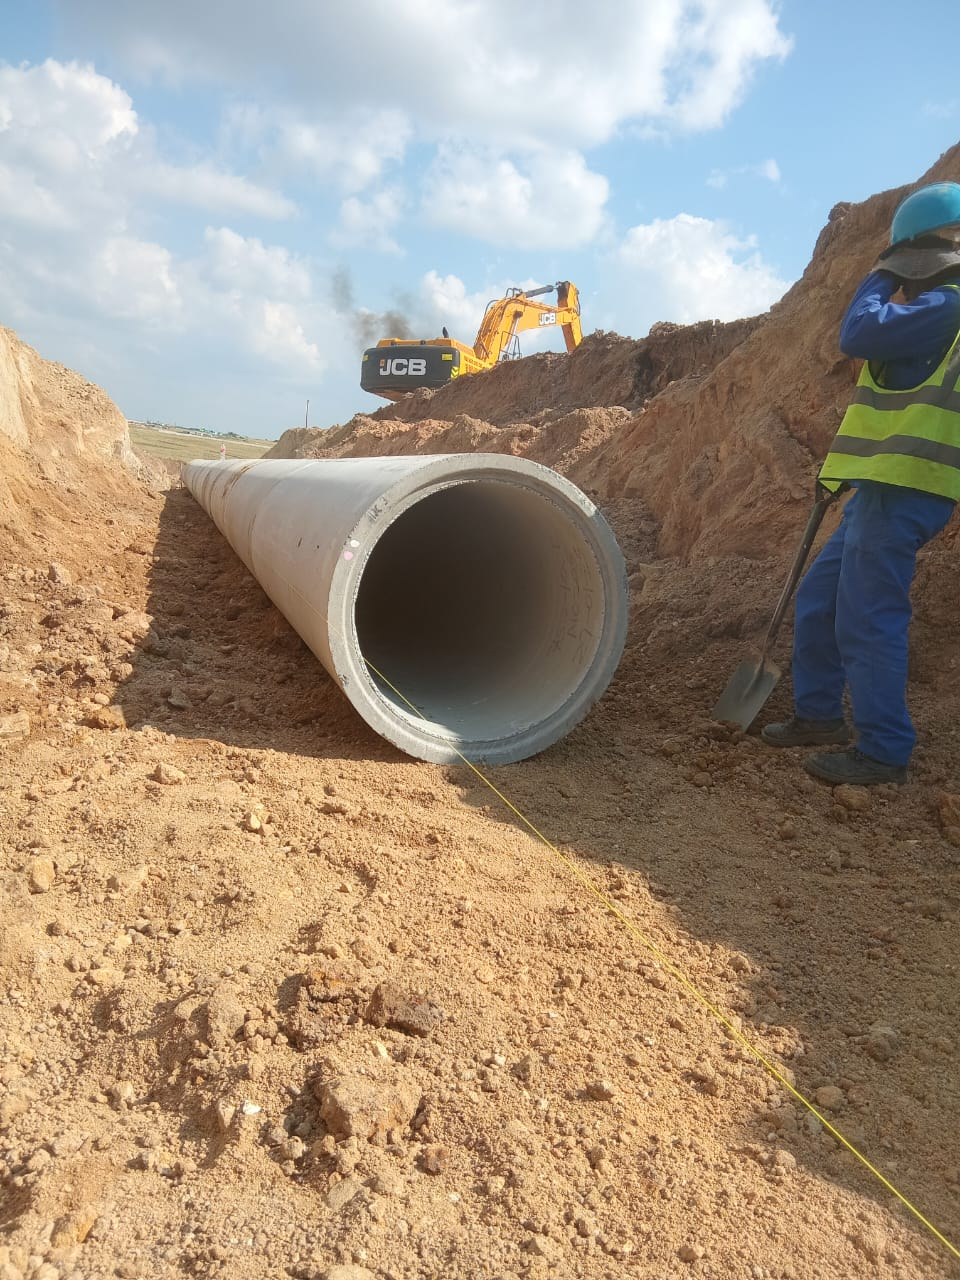
\includegraphics[width=\linewidth, height=2.4cm, keepaspectratio=false]{images/culvert-civil-storm-sewer-pipe.jpeg}
        \centering\vspace{2pt}
        {\fontsize{7pt}{8pt}\selectfont\bfseries\color{mhnavy}Bulk Pipe Reticulation}
    \end{tcolorbox}
\end{minipage}\hfill
\begin{minipage}[t]{0.235\textwidth}
    \begin{tcolorbox}[enhanced, colback=white, colframe=mhlightgray, boxrule=0.7pt, arc=3pt, left=0pt, right=0pt, top=0pt, bottom=3pt]
        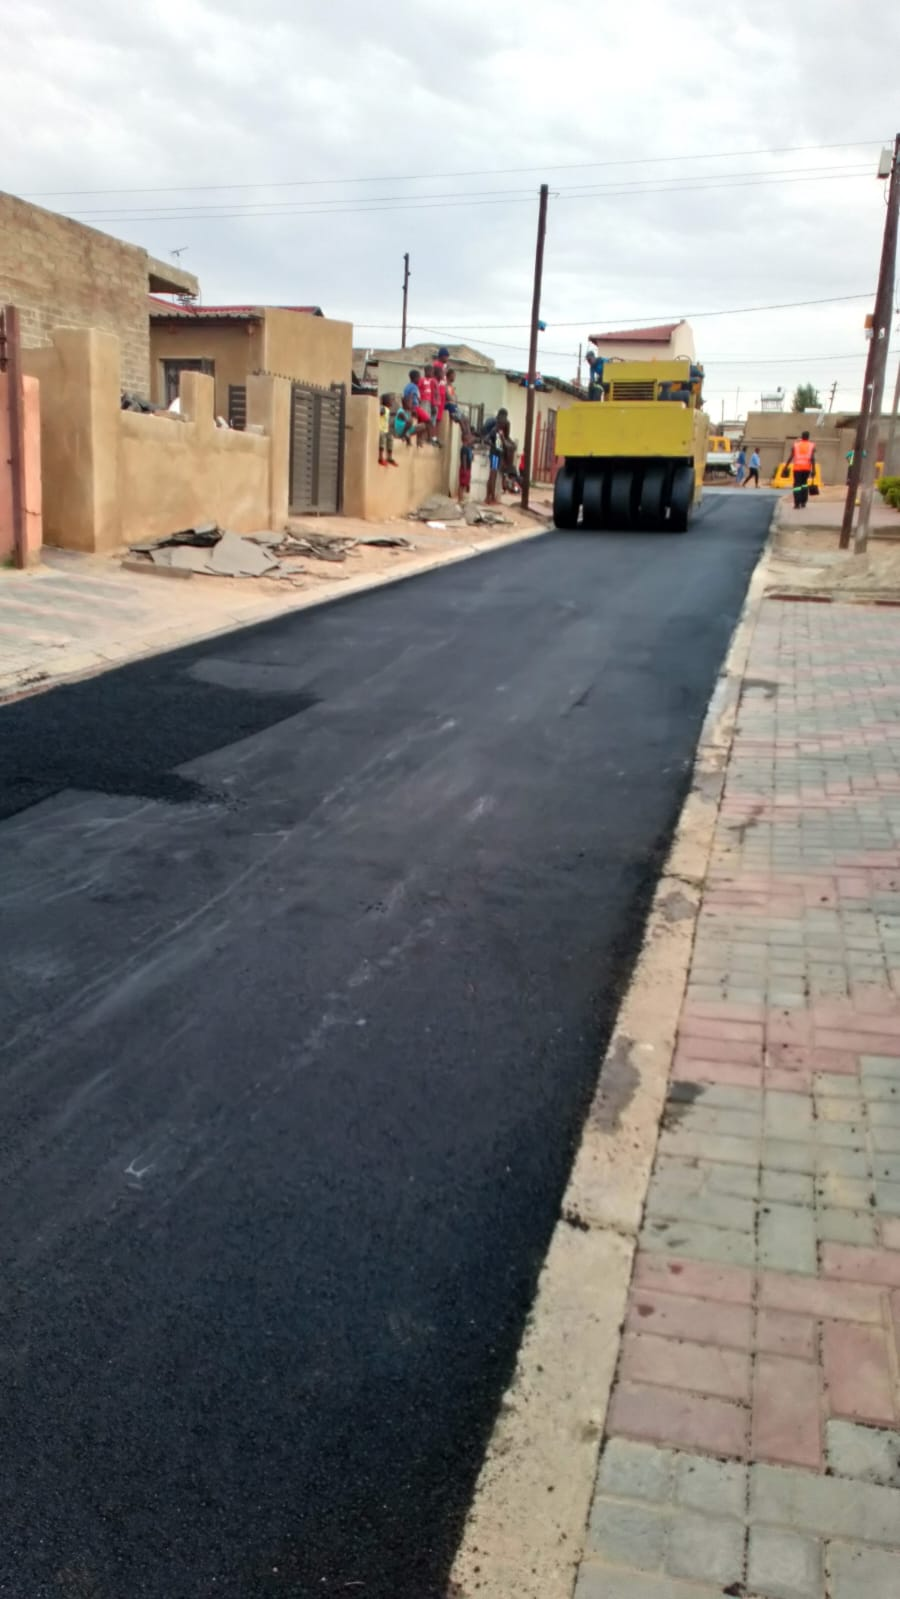
\includegraphics[width=\linewidth, height=2.4cm, keepaspectratio=false]{images/asphalt-photos-1.jpeg}
        \centering\vspace{2pt}
        {\fontsize{7pt}{8pt}\selectfont\bfseries\color{mhtextmuted}LAYERWORKS}\\[1pt]
        {\fontsize{7.5pt}{9pt}\selectfont\bfseries\color{mhnavy}G1 Base \& Asphalt Inlays}
    \end{tcolorbox}
\end{minipage}

\vspace{0.25cm}

{\large\bfseries\color{mhnavy} Verified Civil Engineering \& Road Infrastructure Record}
\vspace{0.15cm}

\renewcommand{\arraystretch}{1.25}
\begin{tabularx}{\textwidth}{@{}p{3.8cm} p{3.2cm} p{1.8cm} X@{}}
\rowcolor{mhnavy}
{\color{white}\bfseries\fontsize{7.8pt}{9.5pt}\selectfont Project \& Contract No.} &
{\color{white}\bfseries\fontsize{7.8pt}{9.5pt}\selectfont Client / Primary Partner} &
{\color{white}\bfseries\fontsize{7.8pt}{9.5pt}\selectfont Period} &
{\color{white}\bfseries\fontsize{7.8pt}{9.5pt}\selectfont Verified Scope of Works Executed} \\
\rowcolor{mhbluelight}
\fontsize{7.5pt}{9pt}\selectfont\bfseries Kaalfontein Phase 3B (JRA/21/157) & \fontsize{7.5pt}{9pt}\selectfont Johannesburg Roads Agency (JRA) & \fontsize{7.5pt}{9pt}\selectfont 2023 -- 2024 & \fontsize{7.5pt}{9pt}\selectfont Dump rock stabilization, sub-base \& base layerworks (1,090m x 6.1m), 600mm stormwater pipelines \& manholes at Reed Fish St. \\
\fontsize{7.5pt}{9pt}\selectfont\bfseries Road D2702 Dwaalboom (RAL/T1171/2021) & \fontsize{7.5pt}{9pt}\selectfont Roads Agency Limpopo / Tarcron Projects & \fontsize{7.5pt}{9pt}\selectfont 2021 -- 2023 & \fontsize{7.5pt}{9pt}\selectfont Heavy pavement layer repairs, asphalt overlay, crack routing, hot-pour bitumen sealing, chip-and-spray \& road markings. \\
\rowcolor{mhbluelight}
\fontsize{7.5pt}{9pt}\selectfont\bfseries Diepsloot Ext 11 Phase 4 (JRA/21/59) & \fontsize{7.5pt}{9pt}\selectfont JRA / Anvisda Plant \& Civils & \fontsize{7.5pt}{9pt}\selectfont 2021 -- 2022 & \fontsize{7.5pt}{9pt}\selectfont Bulk earthworks, subsoil drains, 675mm--1200mm concrete stormwater pipes, roadbed compaction, asphalt surfacing \& paving. \\
\fontsize{7.5pt}{9pt}\selectfont\bfseries Diepsloot Ext 06 Roads (JRA/19/214) & \fontsize{7.5pt}{9pt}\selectfont JRA / SR Construction & \fontsize{7.5pt}{9pt}\selectfont 2019 & \fontsize{7.5pt}{9pt}\selectfont 450mm--1200mm stormwater pipes, catchpits, retaining walls, C4 stabilized layerworks, Figures 8/8C/12 kerbing \& 80mm paving. \\
\rowcolor{mhbluelight}
\fontsize{7.5pt}{9pt}\selectfont\bfseries Diepsloot Phase 4 Zeph Mothopeng (JRA/22/83) & \fontsize{7.5pt}{9pt}\selectfont JRA / Baithusi Trading & \fontsize{7.5pt}{9pt}\selectfont 2023 -- 2024 & \fontsize{7.5pt}{9pt}\selectfont Roadbed prep, cement-stabilized sub-base, G1 crushed base (551m x 5.5m), 600mm concrete pipes, sidewalks \& kerbs. \\
\fontsize{7.5pt}{9pt}\selectfont\bfseries Provincial Road Rehab (DRT23/05/2016) & \fontsize{7.5pt}{9pt}\selectfont Gauteng DRT / Civtek & \fontsize{7.5pt}{9pt}\selectfont Completed & \fontsize{7.5pt}{9pt}\selectfont Kerb inlets with Type 2A covers, cold milling, asphalt patching, concrete driveways, medium-graded surfacing \& bus bays. \\
\end{tabularx}
\renewcommand{\arraystretch}{1}

\vspace{0.15cm}
{\fontsize{7.2pt}{9pt}\selectfont\color{mhtextmuted}
All listed projects are backed by client-signed practical completion certificates and verified contactable engineering references.
}

\clearpage

% =================================================
% PAGE 12 (CONTENT p.9) --- FLAGSHIP PROJECT PORTFOLIO: BUILDING, WATER & BRIDGES
% =================================================

\sectionbanner{PROJECT PORTFOLIO}{Building, Water Reticulation \& Bridge Works}

\noindent
\begin{minipage}[t]{0.235\textwidth}
    \begin{tcolorbox}[enhanced, colback=white, colframe=mhlightgray, boxrule=0.7pt, arc=3pt, left=0pt, right=0pt, top=0pt, bottom=3pt]
        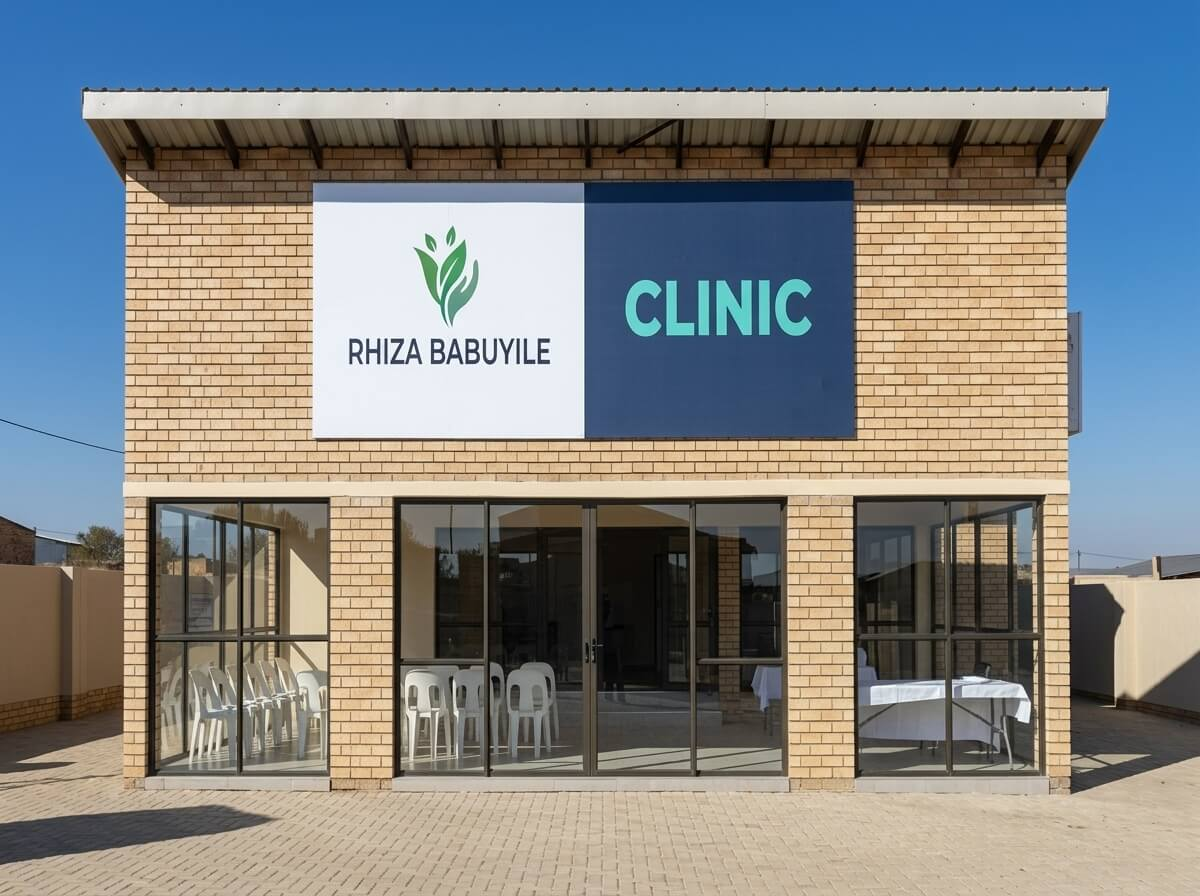
\includegraphics[width=\linewidth, height=2.4cm, keepaspectratio=false]{images/clinic.jpeg}
        \centering\vspace{2pt}
        {\fontsize{7pt}{8pt}\selectfont\bfseries\color{mhtextmuted}HEALTHCARE BUILDS}\\[1pt]
        {\fontsize{7.5pt}{9pt}\selectfont\bfseries\color{mhnavy}Rhiza Community Clinic}
    \end{tcolorbox}
\end{minipage}\hfill
\begin{minipage}[t]{0.235\textwidth}
    \begin{tcolorbox}[enhanced, colback=white, colframe=mhlightgray, boxrule=0.7pt, arc=3pt, left=0pt, right=0pt, top=0pt, bottom=3pt]
        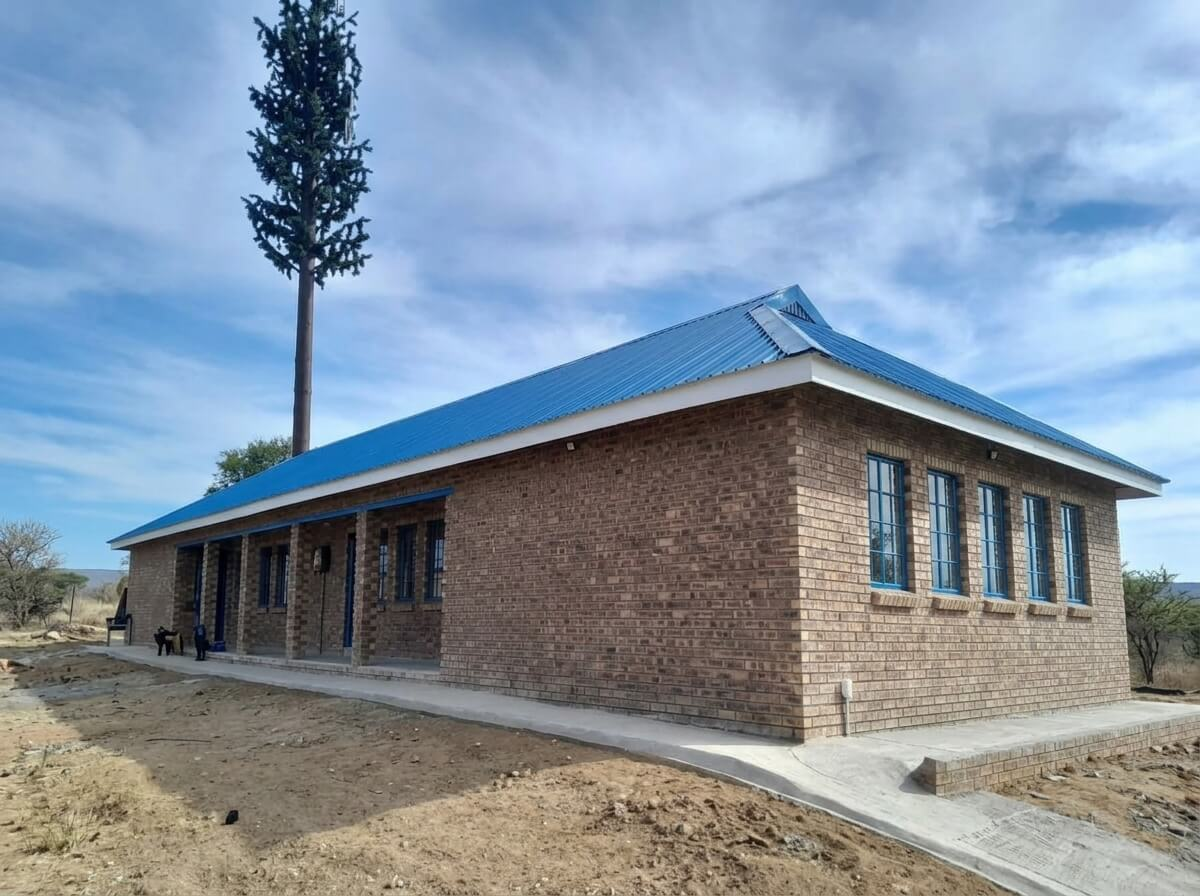
\includegraphics[width=\linewidth, height=2.4cm, keepaspectratio=false]{images/school.jpeg}
        \centering\vspace{2pt}
        {\fontsize{7pt}{8pt}\selectfont\bfseries\color{mhtextmuted}EDUCATIONAL BUILDS}\\[1pt]
        {\fontsize{7.5pt}{9pt}\selectfont\bfseries\color{mhnavy}Classroom Facilities}
    \end{tcolorbox}
\end{minipage}\hfill
\begin{minipage}[t]{0.235\textwidth}
    \begin{tcolorbox}[enhanced, colback=white, colframe=mhlightgray, boxrule=0.7pt, arc=3pt, left=0pt, right=0pt, top=0pt, bottom=3pt]
        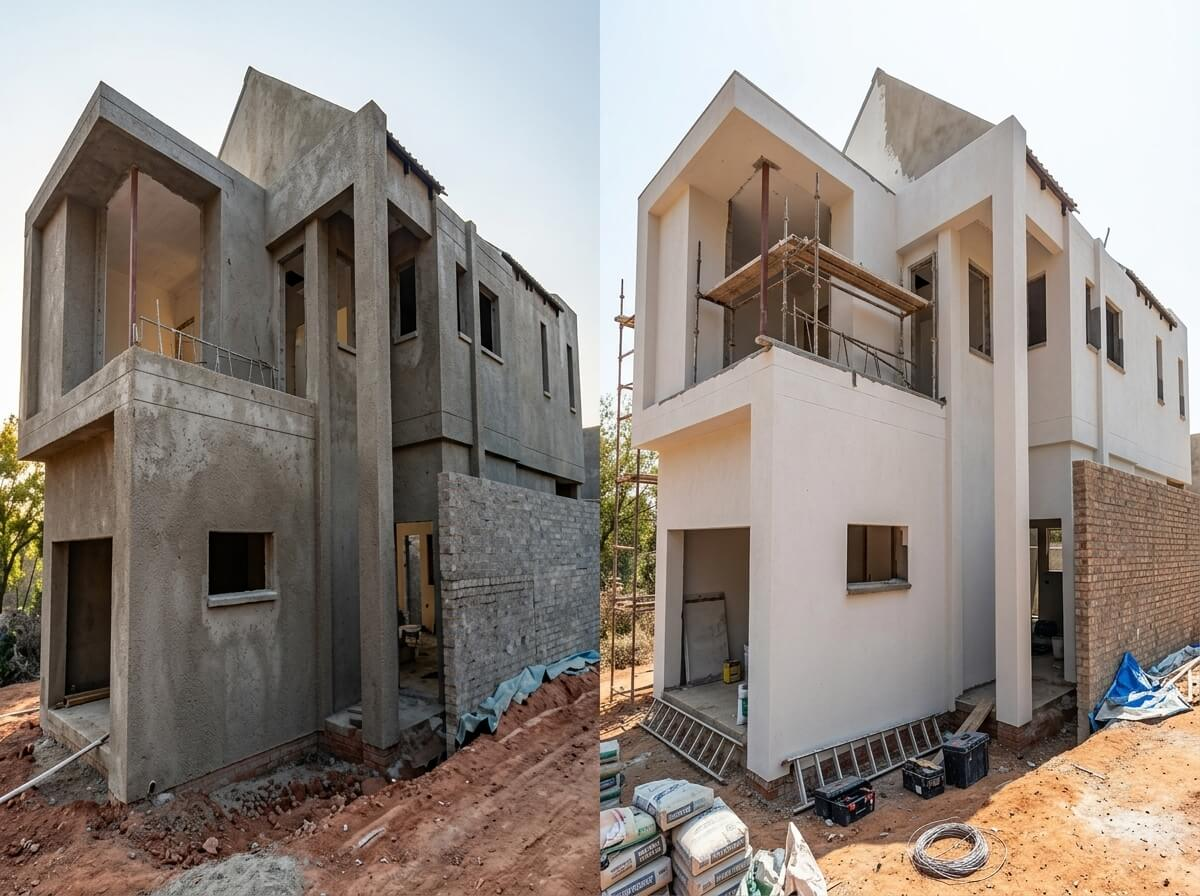
\includegraphics[width=\linewidth, height=2.4cm, keepaspectratio=false]{images/house.jpeg}
        \centering\vspace{2pt}
        {\fontsize{7pt}{8pt}\selectfont\bfseries\color{mhtextmuted}RESIDENTIAL HOUSING}\\[1pt]
        {\fontsize{7.5pt}{9pt}\selectfont\bfseries\color{mhnavy}Double-Storey Builds}
    \end{tcolorbox}
\end{minipage}\hfill
\begin{minipage}[t]{0.235\textwidth}
    \begin{tcolorbox}[enhanced, colback=white, colframe=mhlightgray, boxrule=0.7pt, arc=3pt, left=0pt, right=0pt, top=0pt, bottom=3pt]
        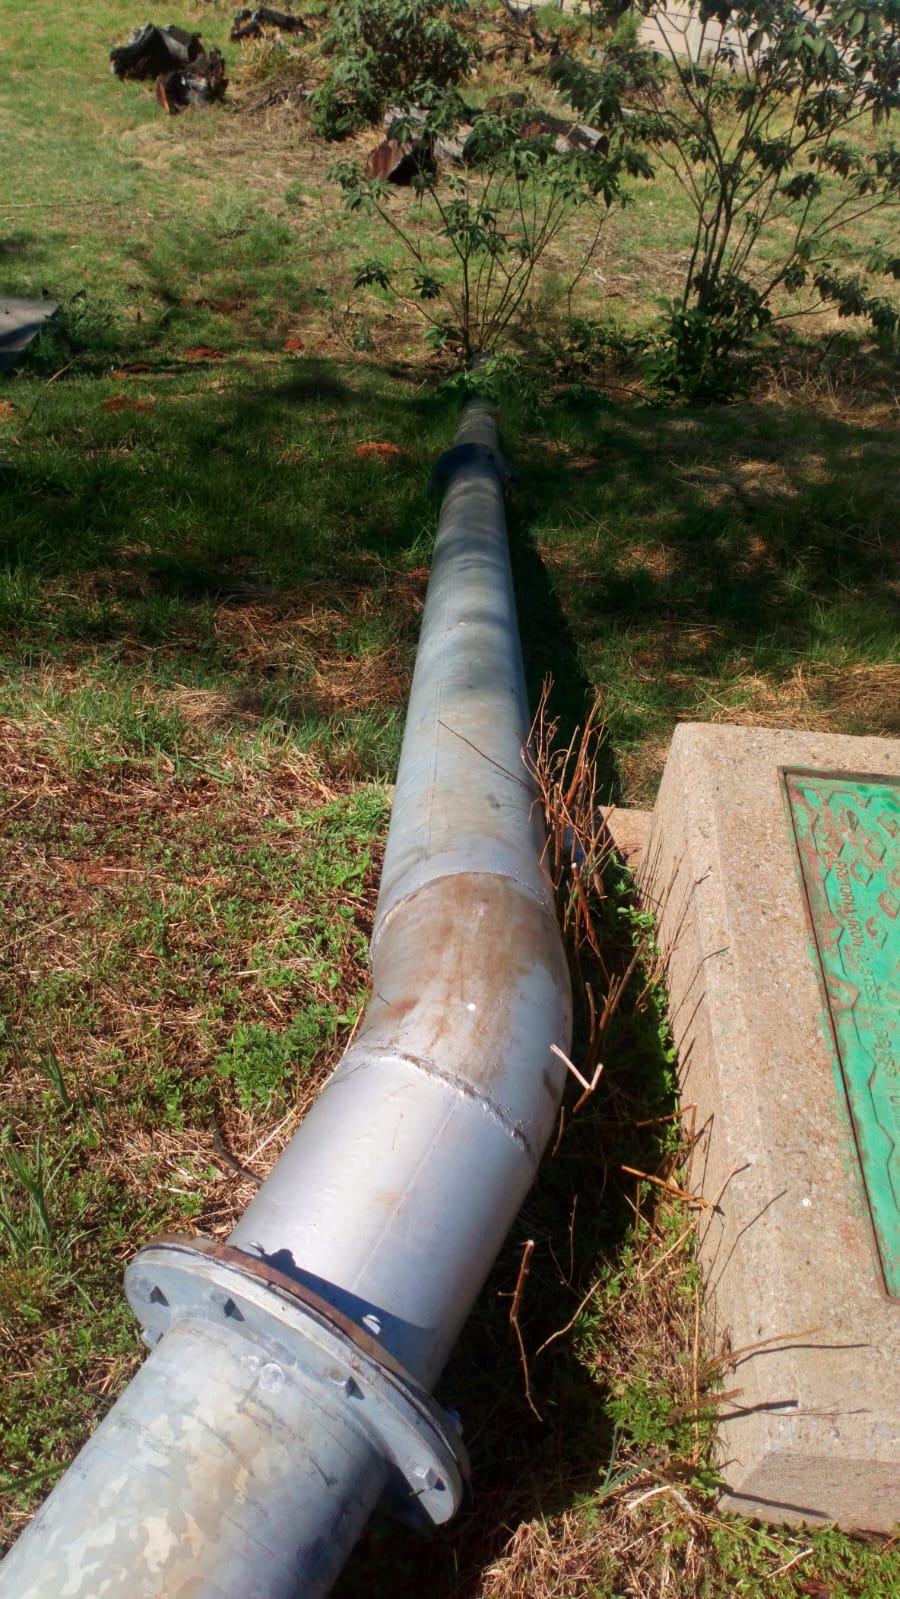
\includegraphics[width=\linewidth, height=2.4cm, keepaspectratio=false]{images/pumphouse-steel-pipe-works-2.jpeg}
        \centering\vspace{2pt}
        {\fontsize{7pt}{8pt}\selectfont\bfseries\color{mhtextmuted}WATER RETICULATION}\\[1pt]
        {\fontsize{7.5pt}{9pt}\selectfont\bfseries\color{mhnavy}Pump Stations \& Valves}
    \end{tcolorbox}
\end{minipage}

\vspace{0.25cm}

{\large\bfseries\color{mhnavy} Verified Building, Water Reticulation \& Bridge Infrastructure Record}
\vspace{0.15cm}

\renewcommand{\arraystretch}{1.25}
\begin{tabularx}{\textwidth}{@{}p{3.8cm} p{3.2cm} p{1.8cm} X@{}}
\rowcolor{mhnavy}
{\color{white}\bfseries\fontsize{7.8pt}{9.5pt}\selectfont Project \& Contract No.} &
{\color{white}\bfseries\fontsize{7.8pt}{9.5pt}\selectfont Client / Primary Partner} &
{\color{white}\bfseries\fontsize{7.8pt}{9.5pt}\selectfont Period} &
{\color{white}\bfseries\fontsize{7.8pt}{9.5pt}\selectfont Verified Scope of Works Executed} \\
\rowcolor{mhbluelight}
\fontsize{7.5pt}{9pt}\selectfont\bfseries Lerome Water Reticulation (014/MKLM/2022/2023) & \fontsize{7.5pt}{9pt}\selectfont Moses Kotane Local Municipality & \fontsize{7.5pt}{9pt}\selectfont 2023 -- 2024 & \fontsize{7.5pt}{9pt}\selectfont Mass rock trenching, uPVC/HDPE bulk potable water pipelines, hydrostatic testing, disinfection \& individual household erf connections. \\
\fontsize{7.5pt}{9pt}\selectfont\bfseries Rhiza Community Clinic Construction & \fontsize{7.5pt}{9pt}\selectfont Rhiza Babalo NGO Healthcare Partner & \fontsize{7.5pt}{9pt}\selectfont 2021 & \fontsize{7.5pt}{9pt}\selectfont Turnkey health clinic: reinforced concrete slab, brickwork, roof trusses, Rhinolite plaster, clinical plumbing, LED wiring \& joinery. \\
\rowcolor{mhbluelight}
\fontsize{7.5pt}{9pt}\selectfont\bfseries Midrand Depot Park Homes (PIK 28/2021-22) & \fontsize{7.5pt}{9pt}\selectfont Pikitup SOC Ltd / City of Johannesburg & \fontsize{7.5pt}{9pt}\selectfont 2022 & \fontsize{7.5pt}{9pt}\selectfont Office plinths, guardhouses, security fencing, complete male/female ablution blocks, bulk water/sewer ties \& waste fleet platforms. \\
\fontsize{7.5pt}{9pt}\selectfont\bfseries Double-Storey Residential -- Samrand & \fontsize{7.5pt}{9pt}\selectfont Sedtrade (Pty) Ltd / Private Developer & \fontsize{7.5pt}{9pt}\selectfont 2022 -- 2023 & \fontsize{7.5pt}{9pt}\selectfont Reinforced concrete foundations, multi-level brick superstructure, suspended slabs, timber roof, plastering, plumbing \& electrical. \\
\rowcolor{mhbluelight}
\fontsize{7.5pt}{9pt}\selectfont\bfseries 4 Classrooms \& Furniture -- Diepsloot West & \fontsize{7.5pt}{9pt}\selectfont Department of Basic Education / SGB & \fontsize{7.5pt}{9pt}\selectfont 2023 & \fontsize{7.5pt}{9pt}\selectfont Turnkey classroom block: reinforced slab, superstructure brickwork, IBR roof, security gates, ceramic tiling, ceilings \& full furniture. \\
\fontsize{7.5pt}{9pt}\selectfont\bfseries Tanganani Ext 51 Civil Works -- Diepsloot & \fontsize{7.5pt}{9pt}\selectfont Civplant Civils / Civtek & \fontsize{7.5pt}{9pt}\selectfont Active & \fontsize{7.5pt}{9pt}\selectfont Class 100D Ogee pipes (450mm--1050mm), 110mm Kaytech subsoil pipes, stepped drop manholes \& standard JRA kerb inlets. \\
\rowcolor{mhbluelight}
\fontsize{7.5pt}{9pt}\selectfont\bfseries Ext 14--19 Access Road \& Bridge (14-2024/25) & \fontsize{7.5pt}{9pt}\selectfont Municipal Infrastructure / Civtek & \fontsize{7.5pt}{9pt}\selectfont Active & \fontsize{7.5pt}{9pt}\selectfont Bridge demolition, portal box culverts, in-situ reinforced concrete bridge deck, abutment wingwalls, road approaches \& kerbing. \\
\fontsize{7.5pt}{9pt}\selectfont\bfseries City of Tshwane Infrastructure JV & \fontsize{7.5pt}{9pt}\selectfont City of Tshwane Metro & \fontsize{7.5pt}{9pt}\selectfont Active & \fontsize{7.5pt}{9pt}\selectfont Joint Venture SEG 41 execution for municipal civil infrastructure upgrades, bulk pipe reticulation, and road surfacing. \\
\end{tabularx}
\renewcommand{\arraystretch}{1}

\clearpage

% =================================================
% PAGE 13 (CONTENT p.10) --- CSI & SOCIO-ECONOMIC TRANSFORMATION
% =================================================

\sectionbanner{SOCIAL IMPACT}{Corporate Social Investment \& Socio-Economic Transformation}

\noindent
\begin{minipage}[t]{0.485\textwidth}
    \servicecard{Local Economic Development (LED)}{Prioritised recruitment of 30\% to 50\% local labour from project host communities, combined with structured on-the-job training in layerworks, pipe laying, concrete shuttering, and machine operations.}
    \vspace{0.22cm}
    \servicecard{Enterprise \& Supplier Development (ESD)}{Ring-fencing specialized trade packages (paving, kerbing, painting, fencing, security) for local emerging SMMEs, paired with practical mentorship in pricing, health and safety, and quality delivery.}
\end{minipage}
\hfill
\begin{minipage}[t]{0.485\textwidth}
    \servicecard{Youth \& Women Empowerment}{Targeted inclusion of female and youth artisans across technical and supervisory site roles, providing certified learnerships, apprenticeship development, and career advancement paths.}
    \vspace{0.22cm}
    \servicecard{Community Infrastructure Aid}{Direct sponsorship of local school facilities (e.g. Diepsloot West Secondary School), community sports tournaments, and donation of building materials for vulnerable community centers.}
\end{minipage}

\vspace{0.35cm}

% Local Skills Transfer Imagery
\noindent
\begin{minipage}[t]{0.485\textwidth}
    \begin{tcolorbox}[enhanced, colback=white, colframe=mhlightgray, boxrule=0.7pt, arc=3pt, left=0pt, right=0pt, top=0pt, bottom=3pt]
        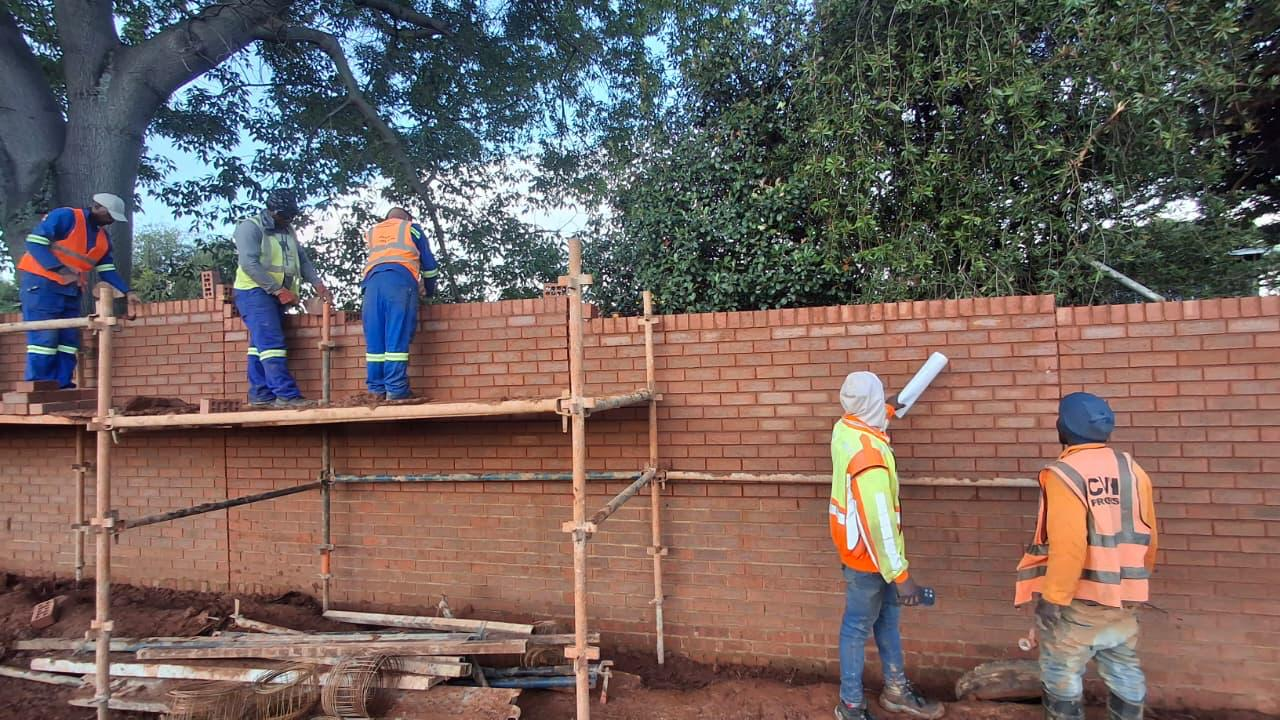
\includegraphics[width=\linewidth, height=3.0cm, keepaspectratio=false]{images/wall-bricklaying.jpeg}
        \centering\vspace{2pt}
        {\fontsize{7.8pt}{9.5pt}\selectfont\bfseries\color{mhnavy}Local Craftsmanship \& Structural Skills Transfer}
    \end{tcolorbox}
\end{minipage}\hfill
\begin{minipage}[t]{0.485\textwidth}
    \begin{tcolorbox}[enhanced, colback=white, colframe=mhlightgray, boxrule=0.7pt, arc=3pt, left=0pt, right=0pt, top=0pt, bottom=3pt]
        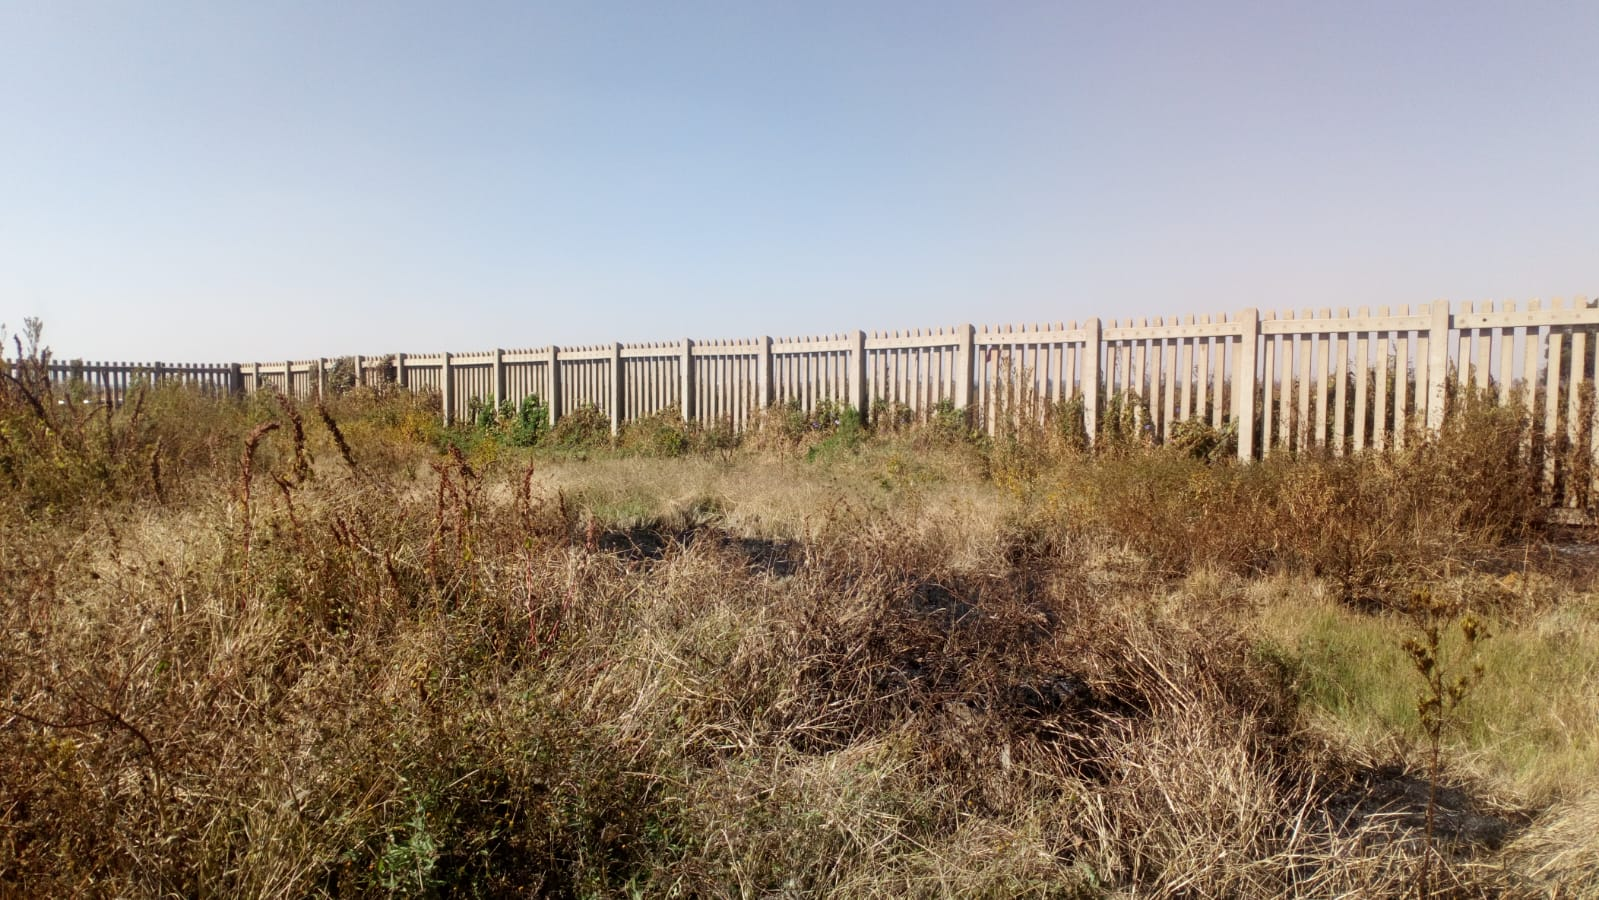
\includegraphics[width=\linewidth, height=3.0cm, keepaspectratio=false]{images/palisade-fencing-1.jpeg}
        \centering\vspace{2pt}
        {\fontsize{7.8pt}{9.5pt}\selectfont\bfseries\color{mhnavy}Security Fencing \& Community Infrastructure}
    \end{tcolorbox}
\end{minipage}

\vspace{0.35cm}

\begin{tcolorbox}[
    enhanced, colback=mhoffwhite, colframe=mhnavy, boxrule=1pt, arc=4pt,
    left=12pt, right=12pt, top=8pt, bottom=8pt
]
    {\fontsize{8.8pt}{12.5pt}\selectfont\color{mhtext}
    \textbf{\color{mhnavy}Our Shared-Value Philosophy:} At Makhaswa Holdings, every contract is treated as a catalyst for sustainable community transformation. Beyond delivering durable infrastructure, we measure our success by the local jobs created, the SMMEs developed, and the technical capabilities left behind in host communities long after practical completion.
    }
\end{tcolorbox}

\clearpage

% =================================================
% PAGE 14 (CONTENT p.11) --- VERIFIED CLIENT REFERENCES & PROJECT DIRECTORY
% =================================================

\sectionbanner{CLIENT REFERENCES}{Contactable Client References \& Project Verification Directory}

\noindent
\begin{minipage}[t]{0.485\textwidth}
    \begin{tcolorbox}[
        enhanced, colback=white, colframe=mhlightgray, boxrule=0.8pt, arc=4pt,
        left=10pt, right=10pt, top=8pt, bottom=8pt,
        borderline west={3pt}{0pt}{mhnavy}
    ]
        {\fontsize{9.5pt}{11.5pt}\selectfont\bfseries\color{mhnavy}\faCheckCircle\ Practical Completion \& QA Sign-Off}\\[3pt]
        {\fontsize{8pt}{11pt}\selectfont\color{mhtext}
        All completed works undergo structured quality assurance sign-offs, including SANAS laboratory concrete compressive strength testing, SANS/AASHTO roadbed compaction verification, and hydrostatic pressure testing on bulk water infrastructure.
        }
    \end{tcolorbox}
\end{minipage}
\hfill
\begin{minipage}[t]{0.485\textwidth}
    \begin{tcolorbox}[
        enhanced, colback=white, colframe=mhlightgray, boxrule=0.8pt, arc=4pt,
        left=10pt, right=10pt, top=8pt, bottom=8pt,
        borderline west={3pt}{0pt}{mhgold}
    ]
        {\fontsize{9.5pt}{11.5pt}\selectfont\bfseries\color{mhnavy}\faFileContract\ Official Tender Due Diligence Directory}\\[3pt]
        {\fontsize{8pt}{11pt}\selectfont\color{mhtext}
        Makhaswa Holdings maintains a verified record of compliant project delivery across municipal, provincial, and private clients. Contactable client references, joint venture partners, and site agents are listed below for official tender evaluation:
        }
    \end{tcolorbox}
\end{minipage}

\vspace{0.3cm}

{\large\bfseries\color{mhnavy} Contactable Client \& Engineering References}
\vspace{0.15cm}

\renewcommand{\arraystretch}{1.25}
\begin{tabularx}{\textwidth}{@{}p{3.8cm} p{2.8cm} p{3.2cm} X@{}}
\rowcolor{mhnavy}
{\color{white}\bfseries\fontsize{7.8pt}{9.5pt}\selectfont Organization} &
{\color{white}\bfseries\fontsize{7.8pt}{9.5pt}\selectfont Contact Person} &
{\color{white}\bfseries\fontsize{7.8pt}{9.5pt}\selectfont Telephone / Email} &
{\color{white}\bfseries\fontsize{7.8pt}{9.5pt}\selectfont Reference Project} \\
\rowcolor{mhbluelight}
\fontsize{7.5pt}{9pt}\selectfont\bfseries Civtek / Civplant Civils & \fontsize{7.5pt}{9pt}\selectfont Paul Bowyer (Site Mgr) & \fontsize{7.5pt}{9pt}\selectfont 012 666 0900 / 082 564 0237 $\bullet$ admin@civtek.co.za & \fontsize{7.5pt}{9pt}\selectfont Tanganani Ext 51, DRT23 Rehab, Bridge Recon \\
\fontsize{7.5pt}{9pt}\selectfont\bfseries Tarcron Projects & \fontsize{7.5pt}{9pt}\selectfont Mr. Makhoshi (Contracts Mgr) & \fontsize{7.5pt}{9pt}\selectfont 015 298 8049 & \fontsize{7.5pt}{9pt}\selectfont RAL/T1171/2021 Road D2702 Dwaalboom \\
\rowcolor{mhbluelight}
\fontsize{7.5pt}{9pt}\selectfont\bfseries Anvisda Plant \& Civils & \fontsize{7.5pt}{9pt}\selectfont Mr. Omen Metani (Site Mgr) & \fontsize{7.5pt}{9pt}\selectfont 071 704 1876 & \fontsize{7.5pt}{9pt}\selectfont JRA/21/59 Diepsloot Ext 11 Phase 4 \\
\fontsize{7.5pt}{9pt}\selectfont\bfseries Baithusi Trading & \fontsize{7.5pt}{9pt}\selectfont Mr. Bophelo Lesia (Site Mgr) & \fontsize{7.5pt}{9pt}\selectfont 068 003 4790 $\bullet$ admin@baithusitrading.co.za & \fontsize{7.5pt}{9pt}\selectfont JRA/22/83 Diepsloot Phase 4 Zeph Mothopeng \\
\rowcolor{mhbluelight}
\fontsize{7.5pt}{9pt}\selectfont\bfseries Johannesburg Roads Agency & \fontsize{7.5pt}{9pt}\selectfont Mr. TB Siboza (Site Agent) & \fontsize{7.5pt}{9pt}\selectfont 011 979 5329 & \fontsize{7.5pt}{9pt}\selectfont JRA/21/157 Kaalfontein Phase 3B \\
\fontsize{7.5pt}{9pt}\selectfont\bfseries SR Construction & \fontsize{7.5pt}{9pt}\selectfont Mr. Sydney Mello (Manager) & \fontsize{7.5pt}{9pt}\selectfont 084 055 7742 & \fontsize{7.5pt}{9pt}\selectfont JRA/19/214 Diepsloot Ext 06 \\
\rowcolor{mhbluelight}
\fontsize{7.5pt}{9pt}\selectfont\bfseries Moses Kotane Municipality & \fontsize{7.5pt}{9pt}\selectfont Mogotsi Kgosiemang (PM) & \fontsize{7.5pt}{9pt}\selectfont 071 395 9004 & \fontsize{7.5pt}{9pt}\selectfont 014/MKLM/2022/2023 Lerome Water Supply \\
\fontsize{7.5pt}{9pt}\selectfont\bfseries Sedtrade (Pty) Ltd & \fontsize{7.5pt}{9pt}\selectfont Mr. Sheeven Bemram & \fontsize{7.5pt}{9pt}\selectfont 071 871 0820 $\bullet$ sheeven@sedtrade.co.za & \fontsize{7.5pt}{9pt}\selectfont Commercial House Facility -- Samrand \\
\rowcolor{mhbluelight}
\fontsize{7.5pt}{9pt}\selectfont\bfseries Pikitup SOC Ltd & \fontsize{7.5pt}{9pt}\selectfont Patrick Mavuso (Site Mgr) & \fontsize{7.5pt}{9pt}\selectfont 012 567 7831 & \fontsize{7.5pt}{9pt}\selectfont PIK 28/2021-22 Midrand Depot Park Homes \\
\fontsize{7.5pt}{9pt}\selectfont\bfseries Diepsloot West Secondary & \fontsize{7.5pt}{9pt}\selectfont Tshilidzi Singo (Principal) & \fontsize{7.5pt}{9pt}\selectfont 010 541 0670 & \fontsize{7.5pt}{9pt}\selectfont 4 Classrooms with Furniture Build \\
\rowcolor{mhbluelight}
\fontsize{7.5pt}{9pt}\selectfont\bfseries Rhiza Babalo NGO & \fontsize{7.5pt}{9pt}\selectfont Thambulo Mabuke (Lead) & \fontsize{7.5pt}{9pt}\selectfont 011 464 5100 & \fontsize{7.5pt}{9pt}\selectfont Construction of Rhiza Community Clinic \\
\end{tabularx}
\renewcommand{\arraystretch}{1}

\clearpage

% =================================================
% PAGE 15 (CONTENT p.12) --- TENDER DUE DILIGENCE, WARRANTIES & BACK COVER
% =================================================
\thispagestyle{empty}

\begin{tikzpicture}[remember picture, overlay]
    \fill[mhnavy] (current page.north west) rectangle (current page.south east);
    \fill[left color=mhnavy, right color=mhnavy2, opacity=0.5] (current page.north west) rectangle (current page.south east);
    \fill[mhgold] (current page.north west) rectangle ([yshift=-0.18cm]current page.north east);
    \fill[mhgold] (current page.south west) rectangle ([yshift=0.18cm]current page.south east);

    % Header Logo Box (Compact & Shifted Upwards with Clean Clearance)
    \node[anchor=north, inner sep=0pt] at ([yshift=-1.0cm]current page.north) {
        \begin{tcolorbox}[
            enhanced, colback=white, colframe=white, boxrule=0pt, arc=4pt,
            left=6pt, right=6pt, top=4pt, bottom=4pt, width=3.8cm, halign=center,
            drop shadow=black!30
        ]
            
\includegraphics[width=3.2cm, keepaspectratio]{images/logo.jpeg}
        \end{tcolorbox}
    };

    % Title & Subtitle (Positioned with clear vertical separation below logo)
    \node[anchor=north, inner sep=0pt] at ([yshift=-4.3cm]current page.north) {
        {\fontsize{18pt}{21pt}\selectfont\bfseries\color{white} TENDER COMPLIANCE \& CONTACT MATRIX}
    };
    \node[anchor=north, inner sep=0pt] at ([yshift=-5.1cm]current page.north) {
        {\fontsize{8.5pt}{11pt}\selectfont\color{mhbluelight}\MakeUppercase{Vendor Due Diligence, Guarantees \& Regional Directory}}
    };

    % Due Diligence & Warranties Split Box
    \node[anchor=north] at ([yshift=-5.9cm]current page.north) {
        \begin{minipage}{0.88\paperwidth}
        \begin{tcolorbox}[
            enhanced, colback=white!6!mhnavy, colframe=white!20!mhnavy, boxrule=0.7pt, arc=4pt,
            left=10pt, right=10pt, top=7pt, bottom=7pt
        ]
            \fontsize{7.2pt}{10.2pt}\selectfont\color{white}
            \begin{minipage}[t]{0.48\linewidth}
                {\fontsize{8pt}{10pt}\selectfont\bfseries\color{mhgold}\faCheckDouble\ Mandatory Tender Pack (Standing Order):}\\[2pt]
                \textcolor{mhgold}{\faCheckCircle}\ CIPC Certificate (K2017/307900/07)\\
                \textcolor{mhgold}{\faCheckCircle}\ Valid SARS TCS PIN (Tax: 9670117176 / VAT: 4840286027)\\
                \textcolor{mhgold}{\faCheckCircle}\ Level 1 B-BBEE SANAS Certificate (135\% Recognition)\\
                \textcolor{mhgold}{\faCheckCircle}\ Active CIDB Proof (CRS: 10153817 -- 8CE / 8ME / 7SB / 7EB)\\
                \textcolor{mhgold}{\faCheckCircle}\ NHBRC Home Builder Certificate (Reg: 4000006217)\\
                \textcolor{mhgold}{\faCheckCircle}\ COIDA Letter of Good Standing (Reg: 990001157115)\\
                \textcolor{mhgold}{\faCheckCircle}\ National Treasury CSD Report (MAAA0584716)
            \end{minipage}
            \hfill
            \begin{minipage}[t]{0.48\linewidth}
                {\fontsize{8pt}{10pt}\selectfont\bfseries\color{mhgold}\faShieldAlt\ Warranties \& Governance Guarantees:}\\[2pt]
                $\bullet$ \textbf{Defects Liability Period:} Standard 12-Month DLP\\
                $\bullet$ \textbf{Performance Bonds:} GCC 2015 / JBCC / FIDIC compliant\\
                $\bullet$ \textbf{NHBRC Housing:} 5-Yr Major Structural / 1-Yr Roof\\
                $\bullet$ \textbf{Contractors Insurance:} CAR \& R20M Public Liability\\
                $\bullet$ \textbf{Bank Confirmation:} FNB Cheque Acc: 62763534445\\
                $\bullet$ \textbf{Branch Code:} 251445 (Pretoria Main Branch)\\
                $\bullet$ \textbf{Signatory:} Lucas Dinga (Chief Executive Officer)
            \end{minipage}
        \end{tcolorbox}
        \end{minipage}
    };

    % Contact detail cards
    \node[anchor=north] at ([yshift=-11.3cm]current page.north) {
        \begin{minipage}{0.88\paperwidth}
        \begin{tcolorbox}[
            enhanced, colback=white!9!mhnavy, colframe=white!25!mhnavy, boxrule=0.7pt, arc=4pt,
            left=12pt, right=12pt, top=8pt, bottom=8pt
        ]
            \fontsize{8.5pt}{13.5pt}\selectfont\color{white}
\begin{tabularx}{\linewidth}{@{}p{4.2cm} X@{}}
\textbf{\color{mhbluelight}\faMapMarkerAlt\ Pretoria Head Office} & 869 Patryshond Street, Garsfontein, Pretoria, 0042 \\
\textbf{\color{mhbluelight}\faMapMarkerAlt\ Midrand Logistics Hub} & Riversands Incubation Hub, 8--12 Incubation Dr, Riverside View \\
\textbf{\color{mhbluelight}\faMapMarkerAlt\ Limpopo Regional Hub} & 197 Dudu Madisha Drive, Chroompark, Mokopane, 0656 \\
\textbf{\color{mhbluelight}\faMapMarkerAlt\ KZN Regional Hub} & 71 Bertha Mkhize Street, Durban Central, Durban, 4001 \\
\textbf{\color{mhbluelight}\faPhoneAlt\ Head Office / Tender Desk} & 012 944 1702 \ $\bullet$ \ \textbf{Midrand Ops:} 011 568 0938 \\
\textbf{\color{mhbluelight}\faWhatsapp\ WhatsApp Direct Hotline} & +27 81 359 8003 (24/7 Site Support) \\
\textbf{\color{mhbluelight}\faEnvelope\ Tenders \& RFQs Email} & tenders@makhaswaholdings.co.za \\
\textbf{\color{mhbluelight}\faEnvelope\ General Inquiries \& Admin} & info@makhaswaholdings.co.za \ $\bullet$ \ admin@makhaswaholdings.co.za \\
\textbf{\color{mhbluelight}\faGlobe\ Official Corporate Website} & \href{https://www.makhaswaholdings.co.za}{\color{mhgold}\underline{www.makhaswaholdings.co.za}} \\
\end{tabularx}
        \end{tcolorbox}
        \end{minipage}
    };

    % Footer credentials strip
    \node[anchor=south, inner sep=0pt] at ([yshift=0.8cm]current page.south) {
        {\fontsize{7.5pt}{9.5pt}\selectfont\color{white!75}
        Makhaswa Holdings (Pty) Ltd \ $\bullet$ \ CIDB Grade 8 CE PE / 8 ME PE \ $\bullet$ \ Level 1 B-BBEE (135\%) \ $\bullet$ \ Reg: 2017/307900/07}
    };
\end{tikzpicture}
\clearpage

\end{document}
